\chapter{Specific requirements}

\section{External interface requirements}

Users are able to utilize all the main functions that the system provides, making them able to access all the information they are granted permission for.
Given such purposes, any device is suitable to make use of all the S\&C functionalities, allowing convenient access through any web browser.

\subsection{User Interfaces}

\begin{figure}[H]
    \centering
    \begin{minipage}{0.45\textwidth}
        \centering
        \fcolorbox{gray}{white}{
            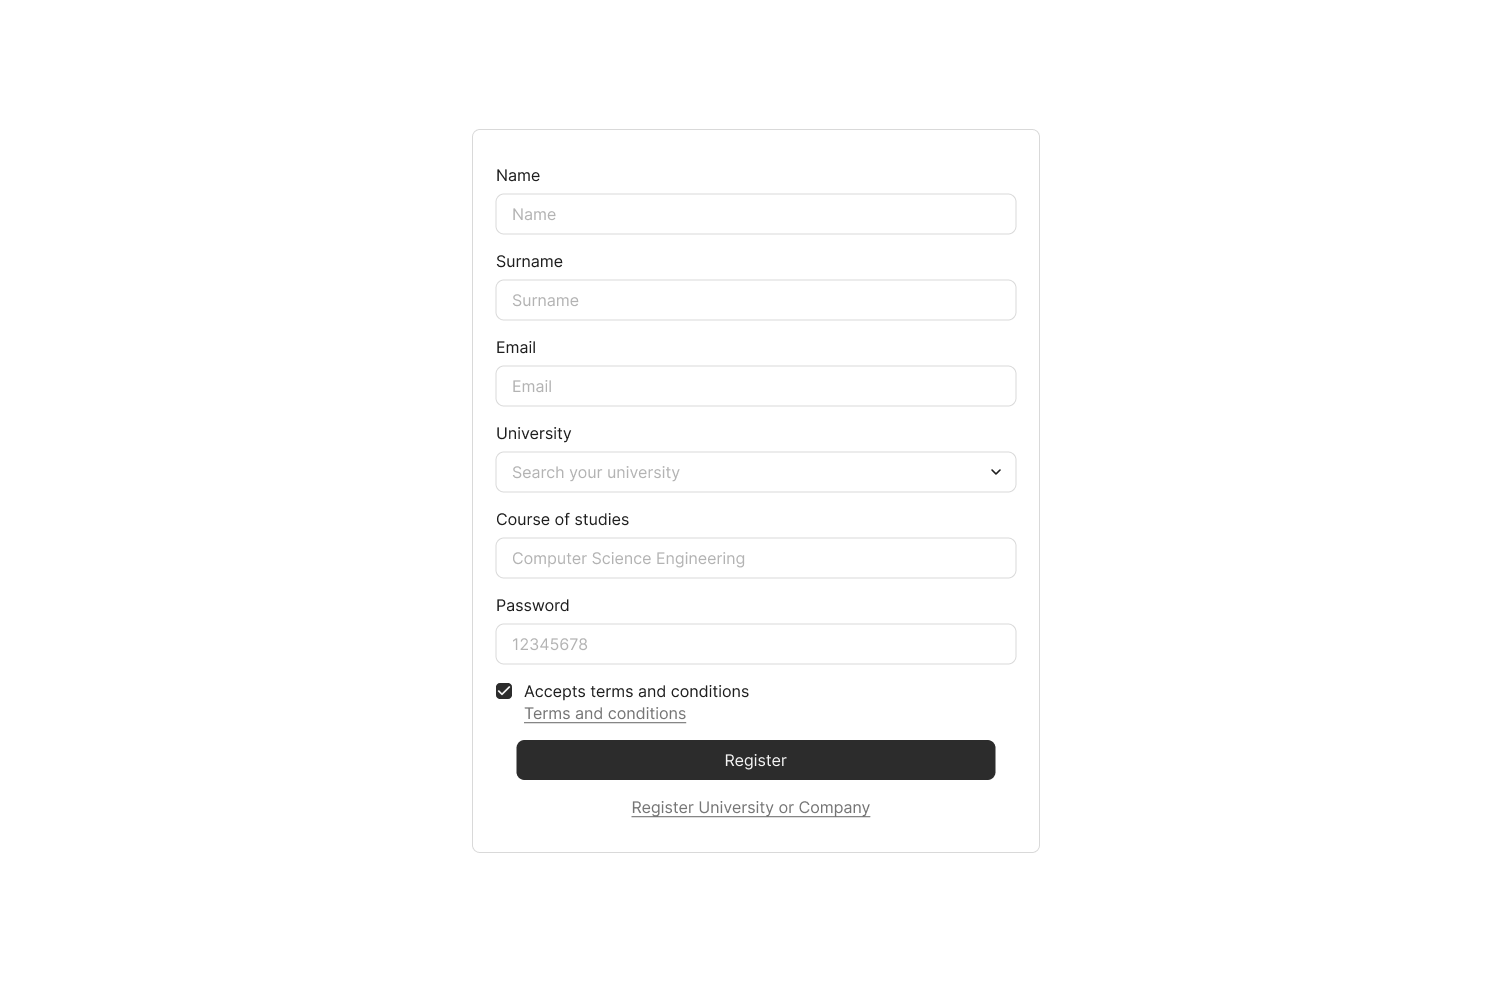
\includegraphics[width=\linewidth]{../../assets/user-interfaces/signup.png}
        }
        \subcaption{Sign up page}
    \end{minipage}
    \hfill
    \begin{minipage}{0.45\textwidth}
        \centering
        \fcolorbox{gray}{white}{
            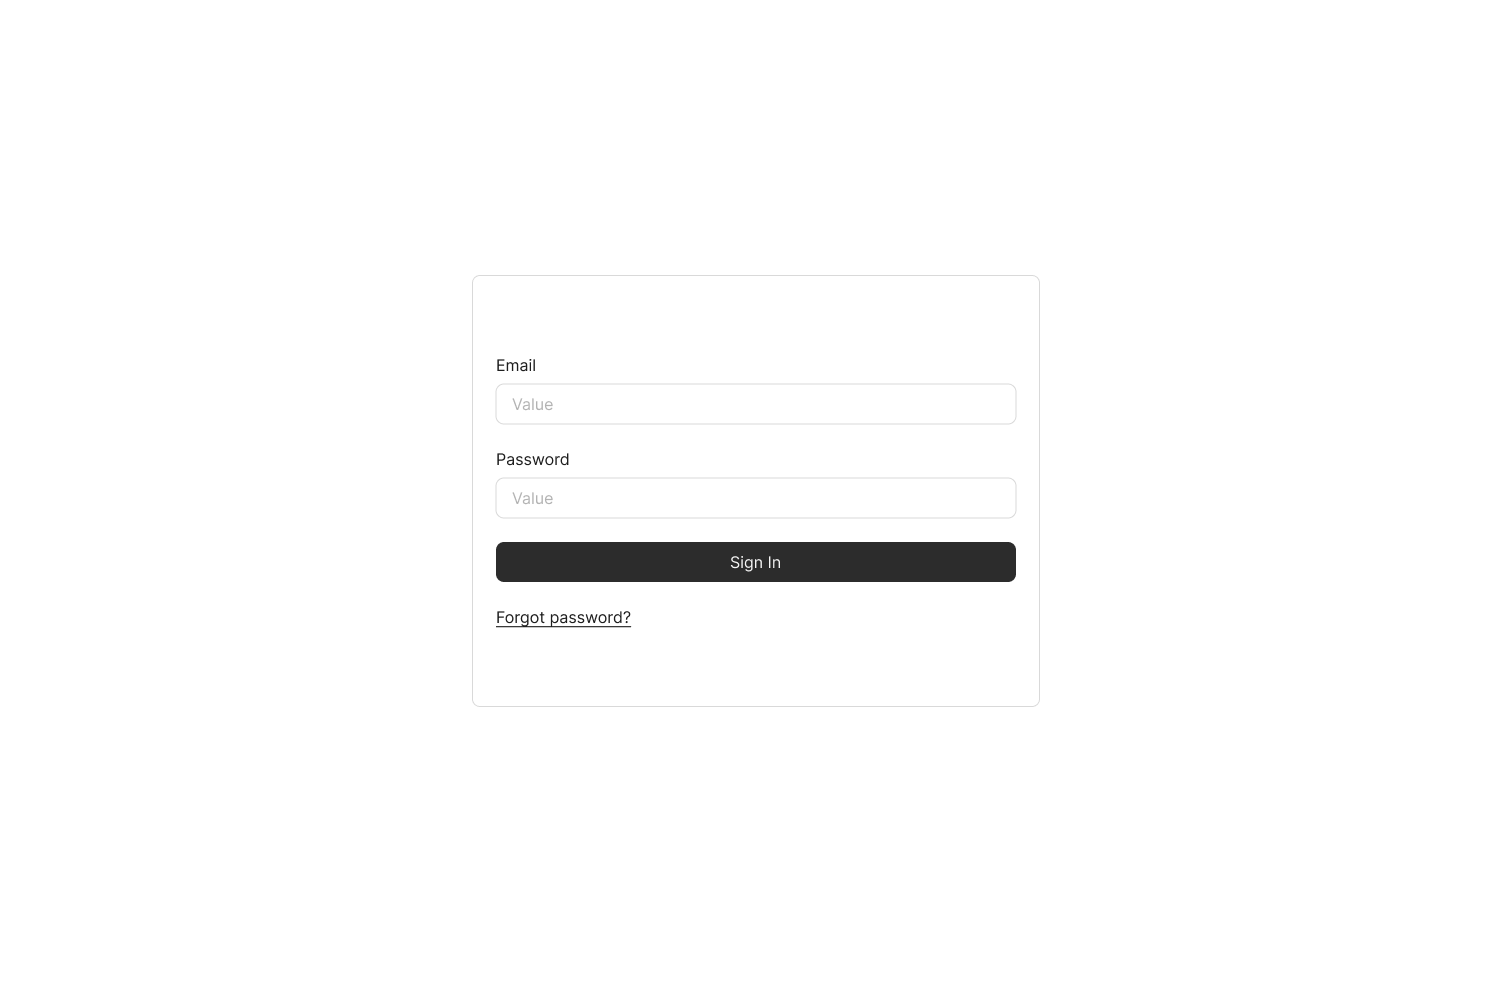
\includegraphics[width=\linewidth]{../../assets/user-interfaces/login.png}
        }
        \subcaption{Log in page}
    \end{minipage}

    \vspace{3em}

    \begin{minipage}{0.45\textwidth}
        \centering
        \fcolorbox{gray}{white}{
            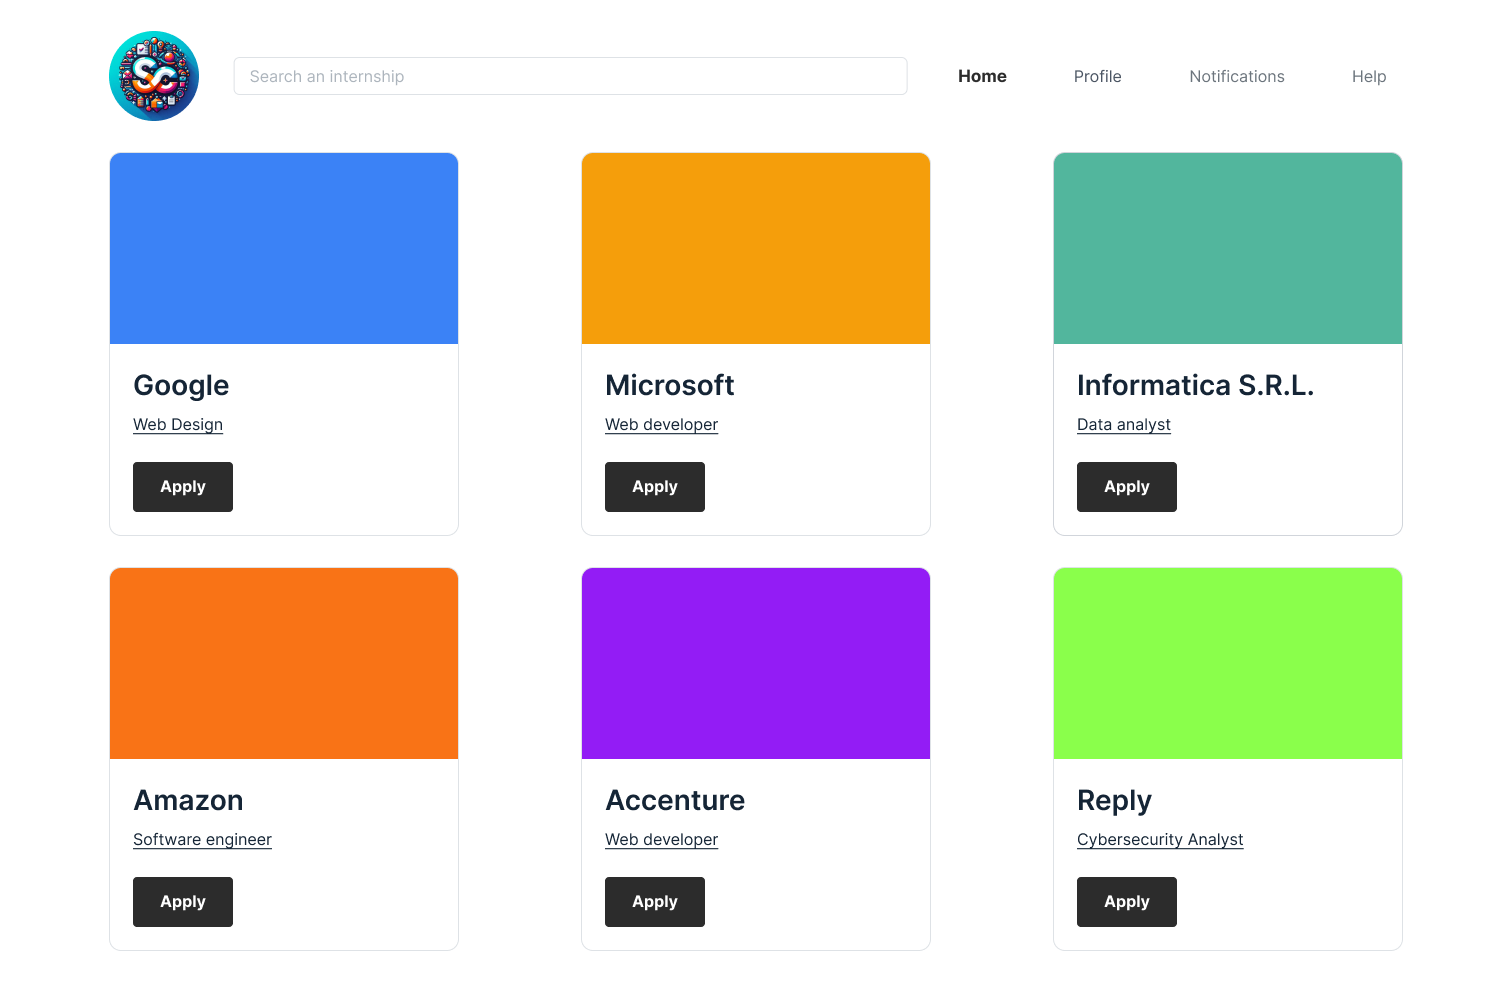
\includegraphics[width=\linewidth]{../../assets/user-interfaces/home.png}
        }
        \subcaption{Home page}
    \end{minipage}
    \hfill
    \begin{minipage}{0.45\textwidth}
        \centering
        \fcolorbox{gray}{white}{
            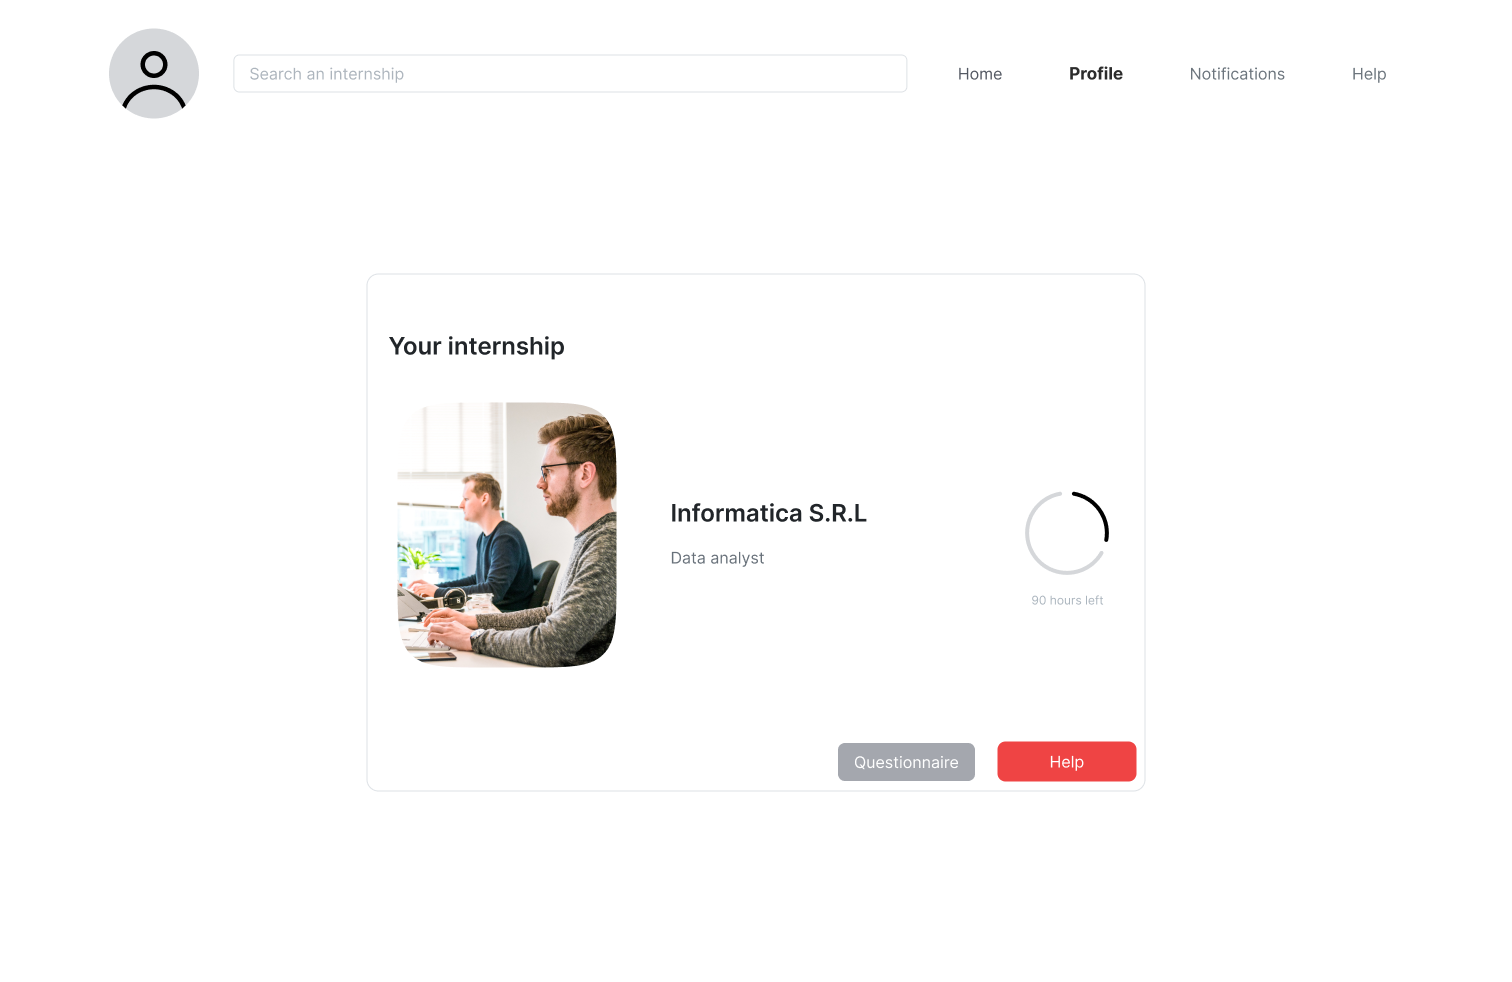
\includegraphics[width=\linewidth]{../../assets/user-interfaces/profile.png}
        }
        \subcaption{Profile page}
    \end{minipage}

    \vspace{3em}

    \begin{minipage}{0.45\textwidth}
        \centering
        \fcolorbox{gray}{white}{
            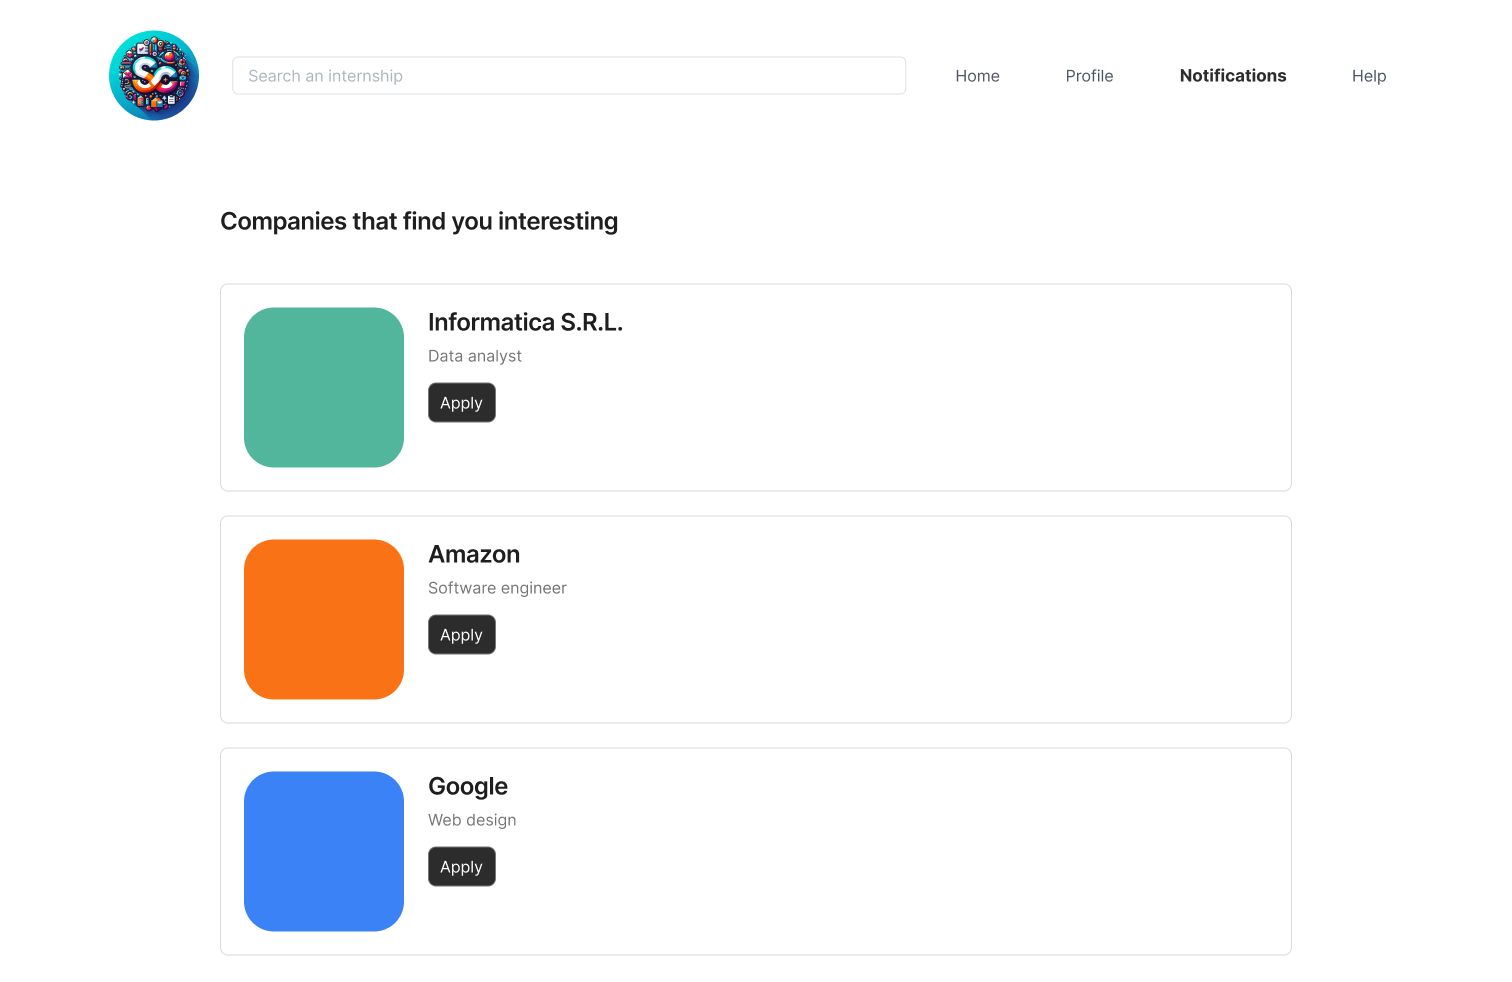
\includegraphics[width=\linewidth]{../../assets/user-interfaces/notifications.png}
        }
        \subcaption{Notifications page}
    \end{minipage}
    \hfill
    \begin{minipage}{0.45\textwidth}
        \centering
        \fcolorbox{gray}{white}{
            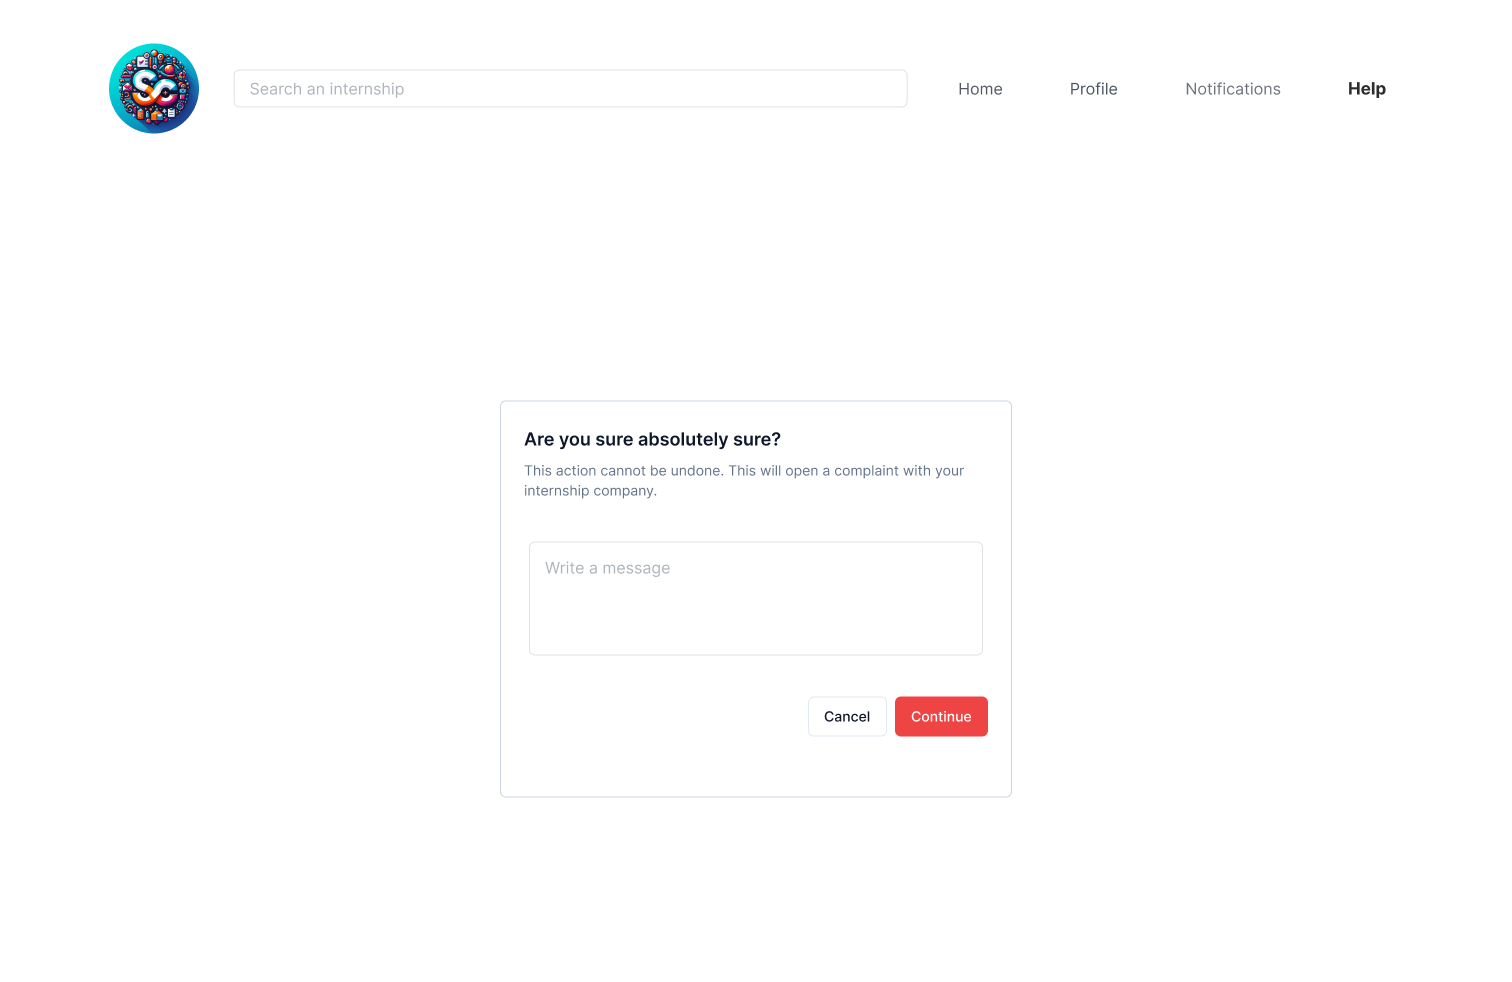
\includegraphics[width=\linewidth]{../../assets/user-interfaces/complaint.png}
        }
        \subcaption{Complaint page}
    \end{minipage}
\end{figure}

\subsection{Hardware Interfaces}

In order be accessed, the platform requires a suitable device with a web browser.

\subsection{Software Interfaces}

The system should integrate an email service, used for the registration process.

\subsection{Communication Interfaces}

The system requires a stable internet connection to work properly.
The connection is used to exchange data between users and the web server, which queries the requested information in a DB.

\section{Functional requirements}

\subsection{Use cases diagrams}

\begin{figure}[H]
    \centering
    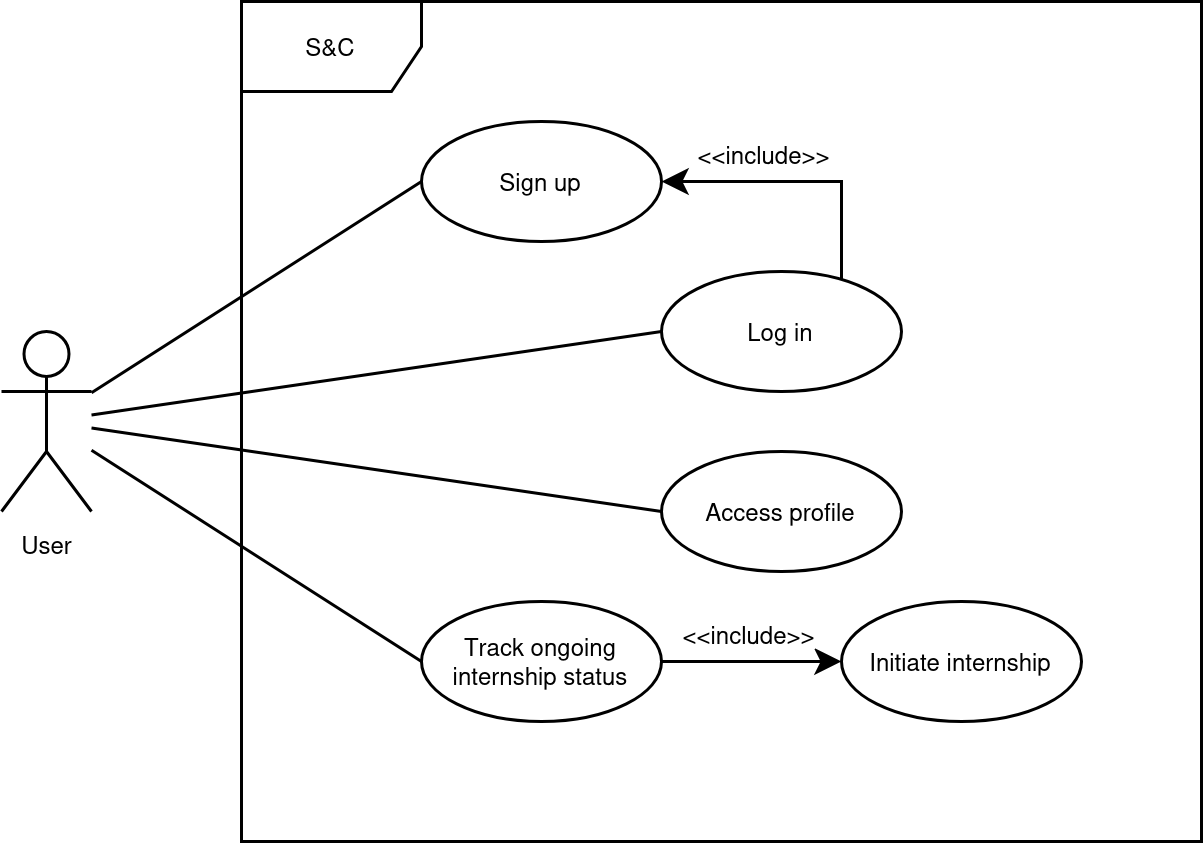
\includegraphics[width=0.3\linewidth]{../../assets/use-case-diagrams/user-common.png}
    \subcaption*{User common use cases}
\end{figure}

\begin{figure}[H]
    \centering
    \begin{minipage}{0.3\textwidth}
        \centering
        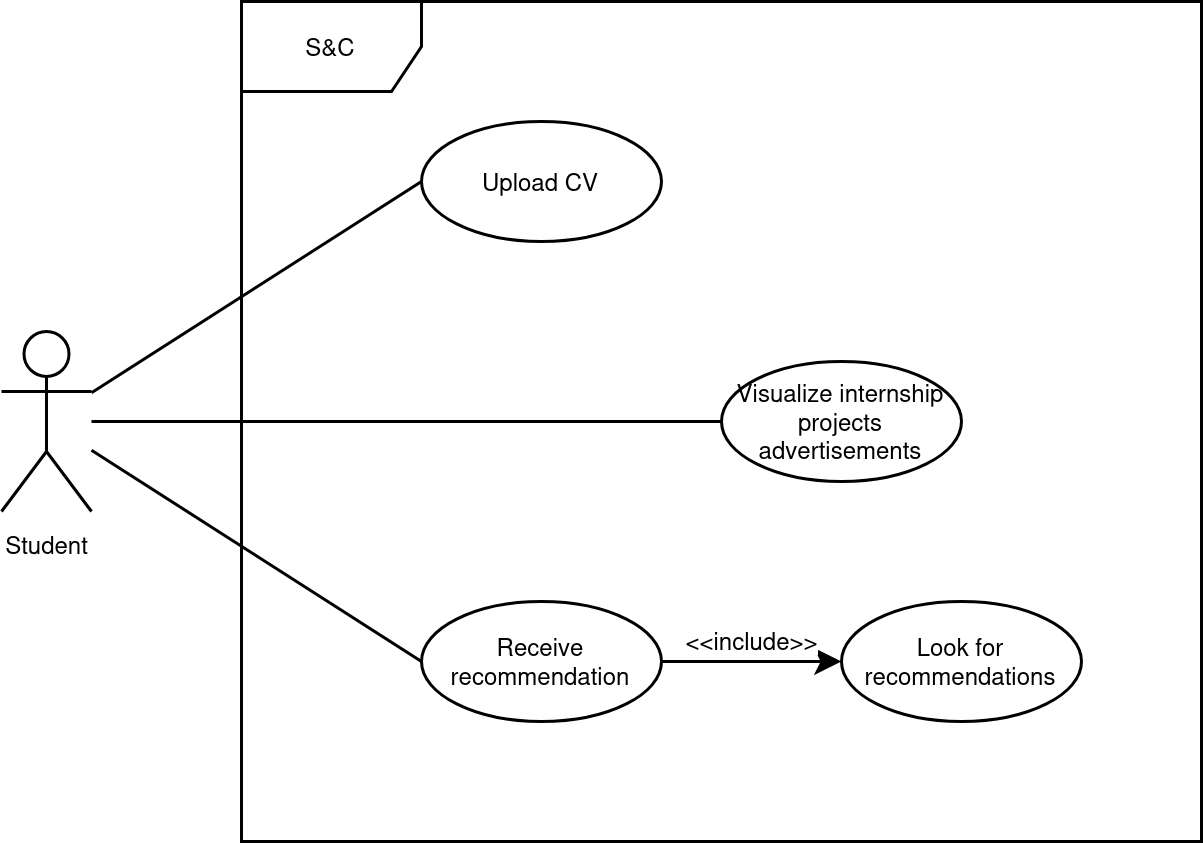
\includegraphics[width=\linewidth]{../../assets/use-case-diagrams/student-unique.png}
        \subcaption*{Student unique use cases}
    \end{minipage}
    \hspace{1in}
    \begin{minipage}{0.3\textwidth}
        \centering
        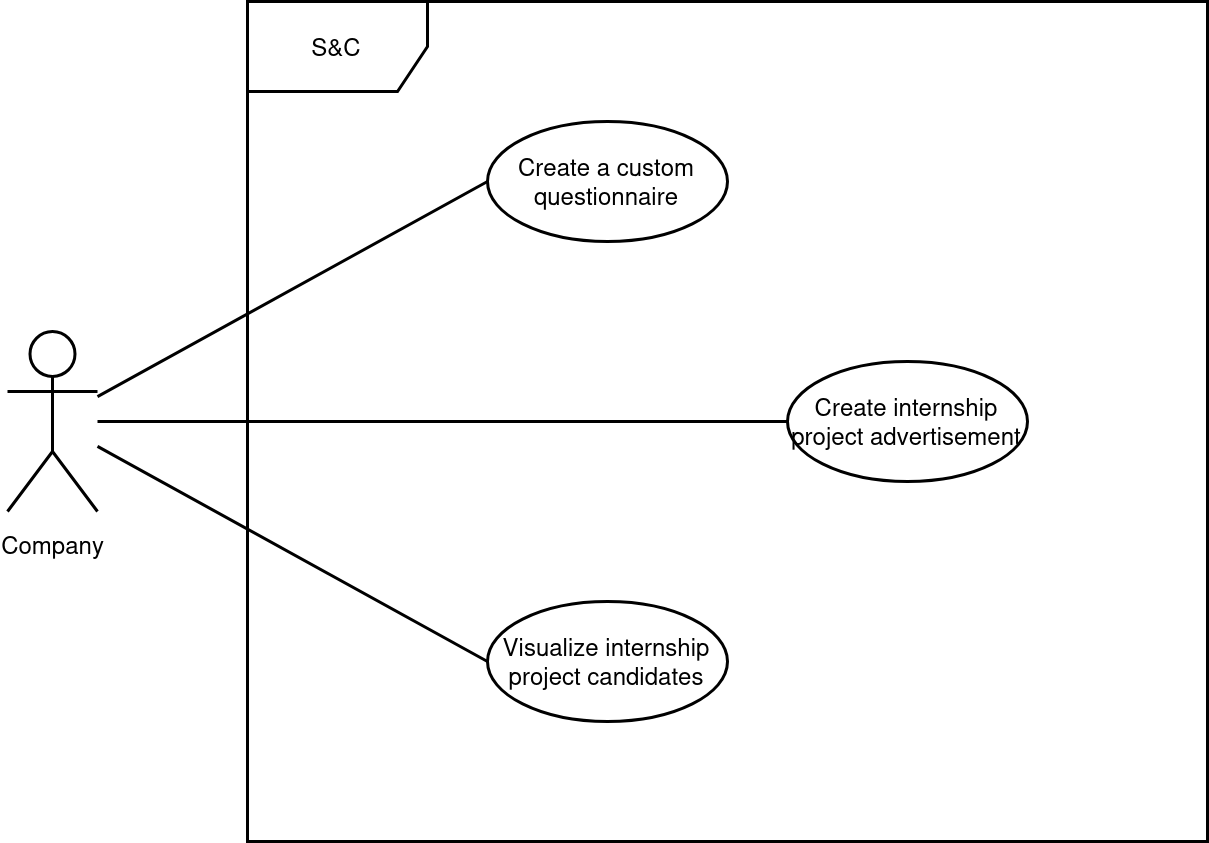
\includegraphics[width=\linewidth]{../../assets/use-case-diagrams/company-unique.png}
        \subcaption*{Company unique use cases}
    \end{minipage}
\end{figure}

\begin{figure}[H]
    \centering
    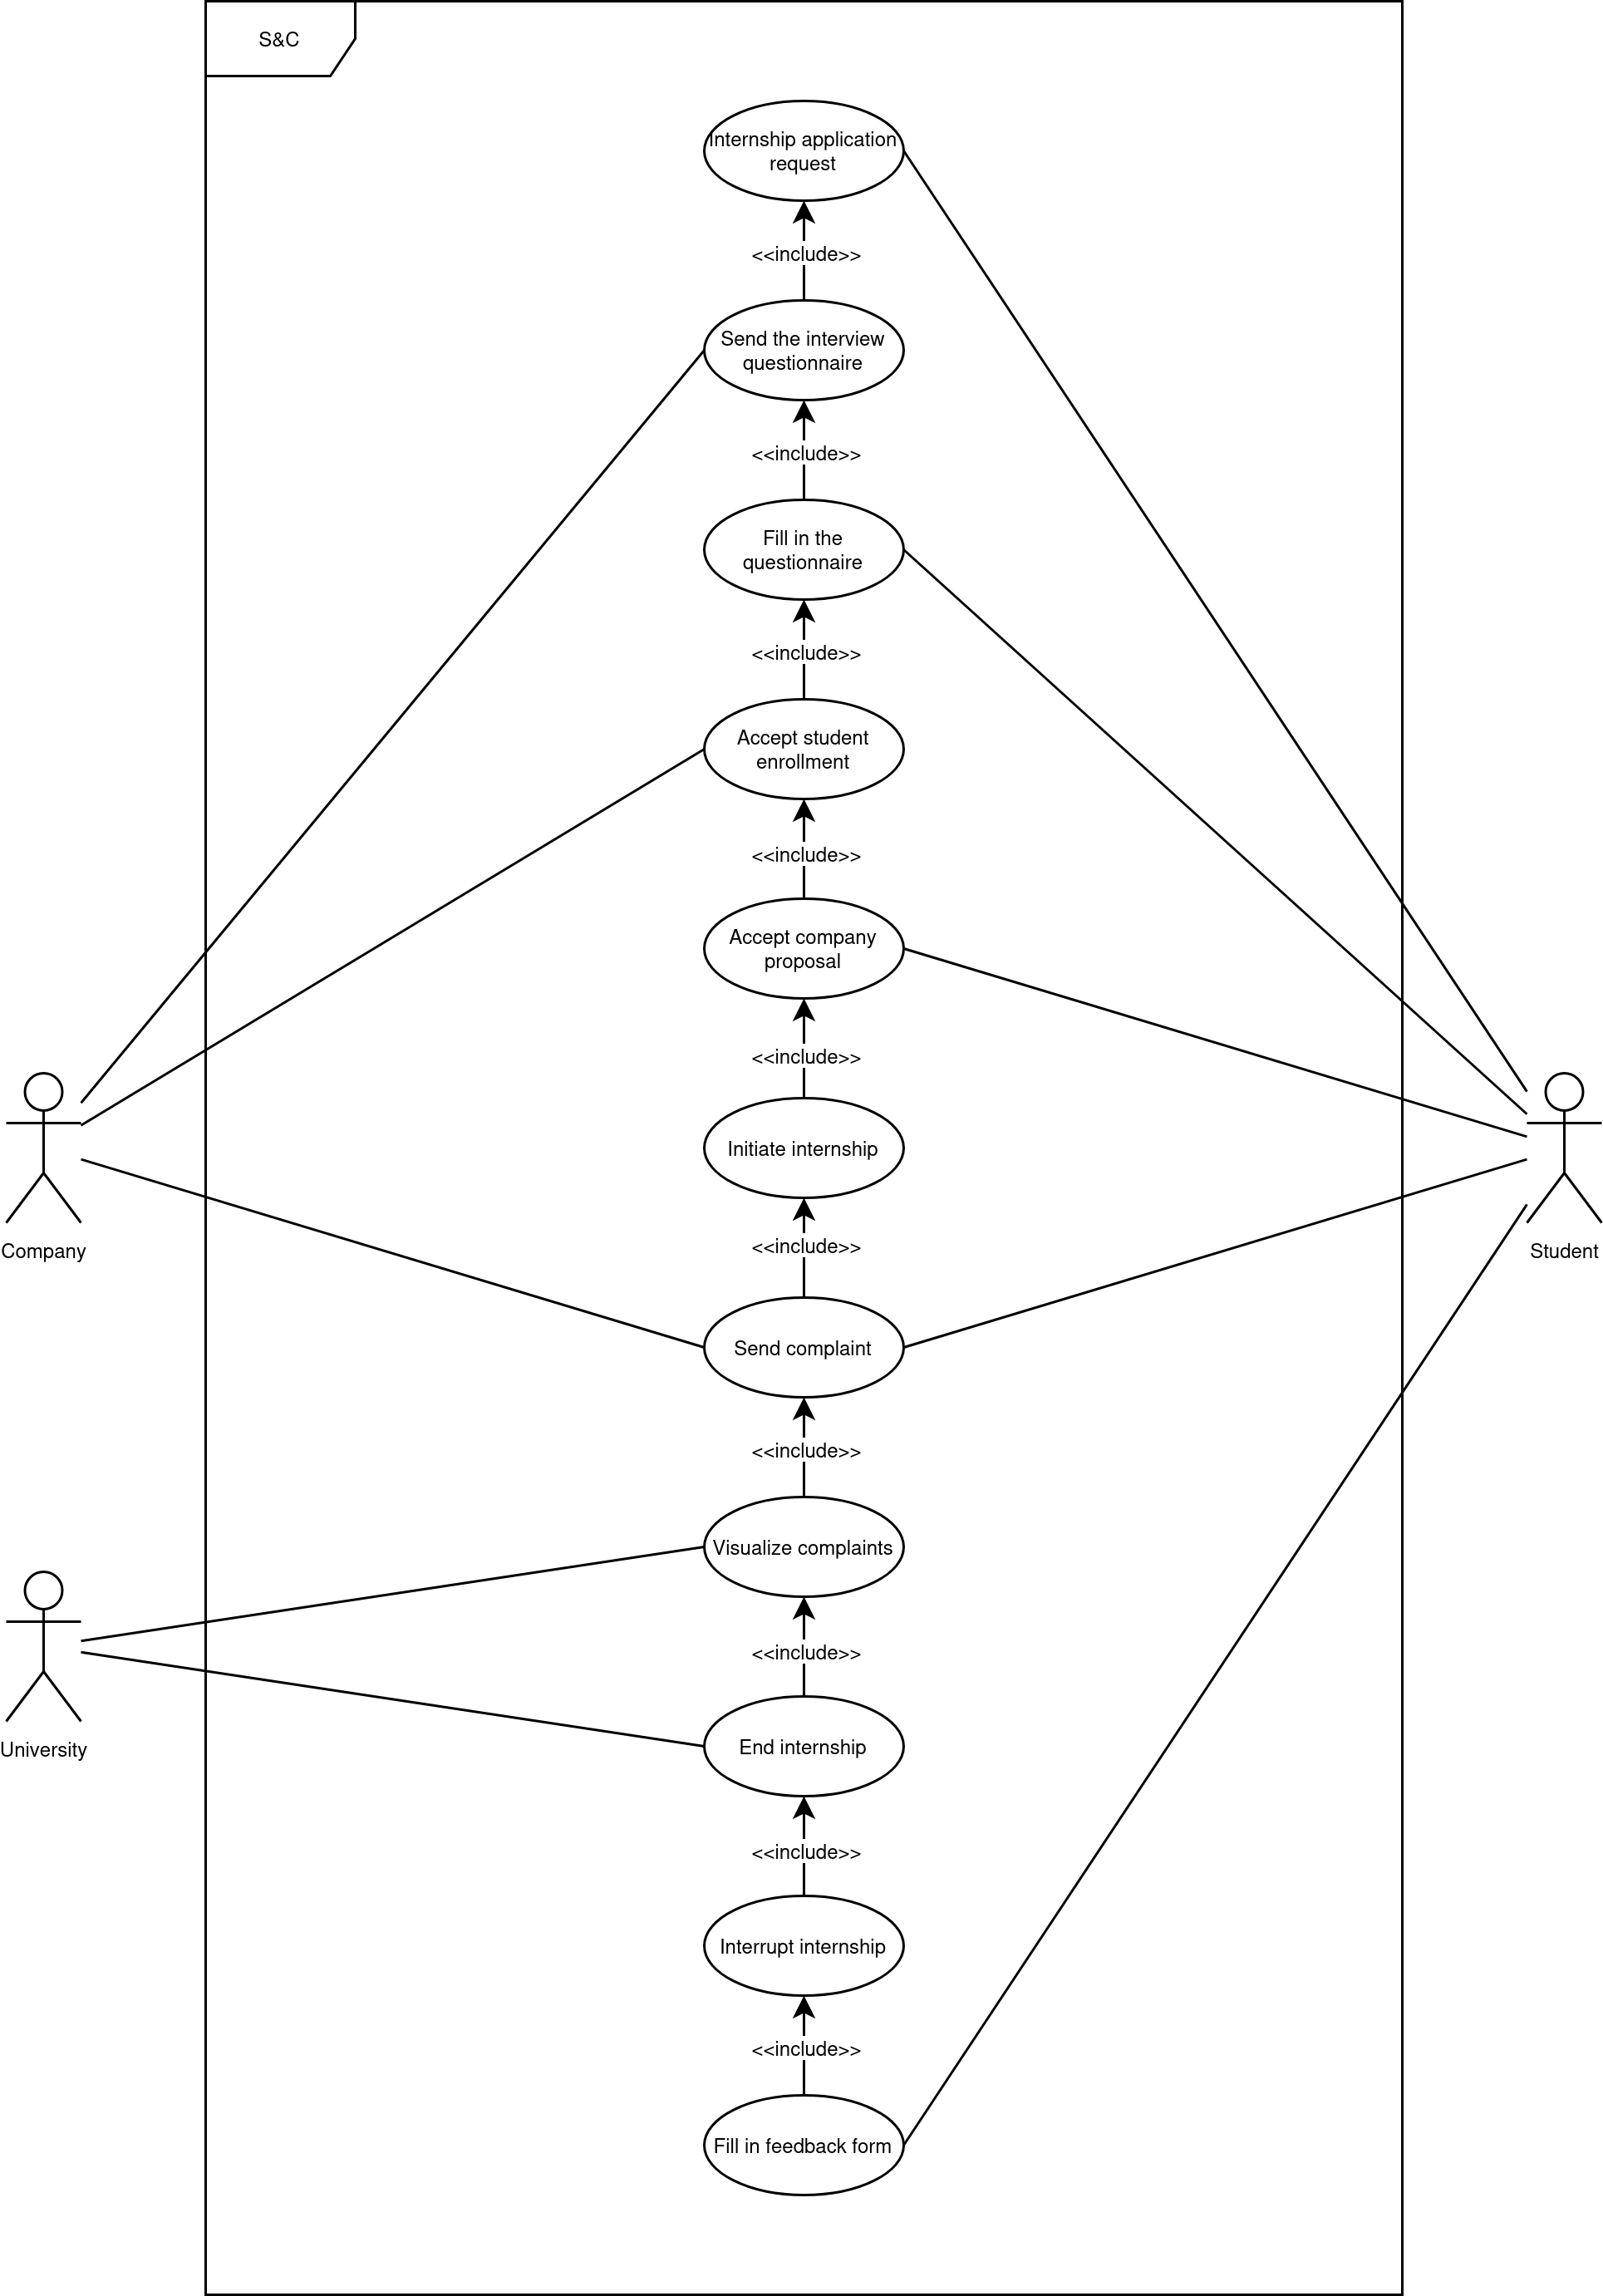
\includegraphics[width=0.8\linewidth]{../../assets/use-case-diagrams/internship-iter.png}
    \subcaption*{Internship iter use cases}
\end{figure}

\subsection{Use cases descriptions}

\begin{enumerate}[label=\textbf{UC\arabic* -}]

\item \subsubsection{StudentSignsUp}

\begin{table}[H]
    \centering
    \begin{tabular}{|l|m{10cm}|}
        \hline \multicolumn{2}{|c|}{\textbf{StudentSignsUp}} \\
        \hline \textbf{Actor} & Student, Students\&Companies, EmailService \\
        \hline \textbf{Entry condition} & The student is not already registered \\
        \hline \textbf{Event flow} &
            \begin{enumerate}[label=\arabic*]
                \item The student opens the sign up page
                \item The student fills in the required information and clicks the sign up button
                \item The platform checks that the information provided is valid
                \item The platform sends an email through the email service to verify the student account
                \item The student verifies the account via the link found in the email
                \item The platform registers the new student account
                \item The platform shows the student feed page
            \end{enumerate} \\
        \hline \textbf{Exit condition} & The student is registered \\
        \hline \textbf{Exceptions} & The student is already registered (3) \\
        \hline
    \end{tabular}
\end{table}

\item \subsubsection{CompanySignsUp}

\begin{table}[H]
    \centering
    \begin{tabular}{|l|m{10cm}|}
        \hline \multicolumn{2}{|c|}{\textbf{CompanySignsUp}} \\
        \hline \textbf{Actor} & Company, Students\&Companies, EmailService \\
        \hline \textbf{Entry condition} & The company is not already registered \\
        \hline \textbf{Event flow} &
            \begin{enumerate}[label=\arabic*]
                \item The company opens the sign up page
                \item The company fills in the required information and clicks the sign up button
                \item The platform checks that the information provided is valid
                \item The platform sends an email through the email service to verify the company account
                \item The company verifies the account via the link found in the email
                \item The platform registers the new company account
                \item The platform shows the company feed page
            \end{enumerate} \\
        \hline \textbf{Exit condition} & The company is registered \\
        \hline \textbf{Exceptions} & The company is already registered (3) \\
        \hline
    \end{tabular}
\end{table}

\item \subsubsection{UserLogsIn}

\begin{table}[H]
    \centering
    \begin{tabular}{|l|m{10cm}|}
        \hline \multicolumn{2}{|c|}{\textbf{UserLogsIn}} \\
        \hline \textbf{Actor} & Student, Company, University, Students\&Companies \\
        \hline \textbf{Entry condition} & User is registered \\
        \hline \textbf{Event flow} &
            \begin{enumerate}[label=\arabic*]
                \item The user opens the log in page
                \item The user enters its credentials and clicks the log in button
                \item The platform checks that the account exists and the credentials are correct
                \item The platform shows the home page
            \end{enumerate} \\
        \hline \textbf{Exit condition} & The user is logged in \\
        \hline \textbf{Exceptions} & The student is not registered (3) \\
        \hline
    \end{tabular}
\end{table}

\item \subsubsection{StudentUploadsCV}

\begin{table}[H]
    \centering
    \begin{tabular}{|l|m{10cm}|}
        \hline \multicolumn{2}{|c|}{\textbf{StudentUploadsCV}} \\
        \hline \textbf{Actor} & Student, Students\&Companies \\
        \hline \textbf{Entry condition} & The student is logged in \\
        \hline \textbf{Event flow} &
            \begin{enumerate}[label=\arabic*]
                \item The student opens the profile page
                \item The student clicks the upload CV button
                \item The student chooses the CV file and lets it upload
                \item The platform receives the file and stores it
                \item The platform shows the student profile page
            \end{enumerate} \\
        \hline \textbf{Exit condition} & The student profile page shows the new CV \\
        \hline \textbf{Exceptions} & None \\
        \hline
    \end{tabular}
\end{table}

\item \subsubsection{CompanyCreatesAdvertisement}

\begin{table}[H]
    \centering
    \begin{tabular}{|l|m{10cm}|}
        \hline \multicolumn{2}{|c|}{\textbf{CompanyCreatesAdvertisement}} \\
        \hline \textbf{Actor} & Company, Students\&Companies \\
        \hline \textbf{Entry condition} & The company is logged in \\
        \hline \textbf{Event flow} &
            \begin{enumerate}[label=\arabic*]
                \item The company opens the home page and clicks the create advertisement button
                \item The company writes out the advertisement details and clicks the post button
                \item The platform receives the advertisements details and stores it
                \item The platform shows the company home page
            \end{enumerate} \\
        \hline \textbf{Exit condition} & The advertisements can be found in the students feed \\
        \hline \textbf{Exceptions} & None \\
        \hline
    \end{tabular}
\end{table}

\item \subsubsection{StudentVisualizesAdvertisements}

\begin{table}[H]
    \centering
    \begin{tabular}{|l|m{10cm}|}
        \hline \multicolumn{2}{|c|}{\textbf{StudentVisualizesAdvertisements}} \\
        \hline \textbf{Actor} & Student, Students\&Companies \\
        \hline \textbf{Entry condition} & The student is logged in \\
        \hline \textbf{Event flow} &
            \begin{enumerate}[label=\arabic*]
                \item The student opens the feed page
                \item The platform searches suitable advertisements to show
                \item The platform sends the advertisements list to the student
                \item The student feed page shows the received list
            \end{enumerate} \\
        \hline \textbf{Exit condition} & The student visualizes interesting advertisements in the feed \\
        \hline \textbf{Exceptions} & None \\
        \hline
    \end{tabular}
\end{table}

\item \subsubsection{CompanyVisualizesCandidates}

\begin{table}[H]
    \centering
    \begin{tabular}{|l|m{10cm}|}
        \hline \multicolumn{2}{|c|}{\textbf{CompanyVisualizesCandidates}} \\
        \hline \textbf{Actor} & Company, Students\&Companies \\
        \hline \textbf{Entry condition} & The company is logged in \\
        \hline \textbf{Event flow} &
            \begin{enumerate}[label=\arabic*]
                \item The company opens the feed page
                \item The platform searches suitable students to show
                \item The platform sends the students list to the company
                \item The company feed page shows the received list
            \end{enumerate} \\
        \hline \textbf{Exit condition} & The company visualizes potential students in the feed \\
        \hline \textbf{Exceptions} & None \\
        \hline
    \end{tabular}
\end{table}

\item \subsubsection{CompanyCreatesQuestionnaire}

\begin{table}[H]
    \centering
    \begin{tabular}{|l|m{10cm}|}
        \hline \multicolumn{2}{|c|}{\textbf{CompanyCreatesQuestionnaire}} \\
        \hline \textbf{Actor} & Company, Students\&Companies \\
        \hline \textbf{Entry condition} & The company is logged in \\
        \hline \textbf{Event flow} &
            \begin{enumerate}[label=\arabic*]
                \item The company opens the home page and clicks the create questionnaire button
                \item The company builds the questionnaire form and clicks the save button
                \item The platform receives the questionnaire form and stores it
                \item The platform shows the company home page
            \end{enumerate} \\
        \hline \textbf{Exit condition} & The questionnaire can be sent to students who have applied \\
        \hline \textbf{Exceptions} & None \\
        \hline
    \end{tabular}
\end{table}

\item \subsubsection{StudentFillsQuestionnaire}

\begin{table}[H]
    \centering
    \begin{tabular}{|l|m{10cm}|}
        \hline \multicolumn{2}{|c|}{\textbf{StudentFillsQuestionnaire}} \\
        \hline \textbf{Actor} & Student, Students\&Companies \\
        \hline \textbf{Entry condition} & The student has received a questionnaire to fill \\
        \hline \textbf{Event flow} &
            \begin{enumerate}[label=\arabic*]
                \item The student opens the notifications page
                \item The student opens the questionnaire that the company has sent
                \item The student fills the questionnaire form and clicks the submit button
                \item The platform sends the filled questionnaire to the company
            \end{enumerate} \\
        \hline \textbf{Exit condition} & The company receives the filled questionnaire \\
        \hline \textbf{Exceptions} & None \\
        \hline
    \end{tabular}
\end{table}

\item \subsubsection{CompanyAcceptsStudentEnrollment}

\begin{table}[H]
    \centering
    \begin{tabular}{|l|m{10cm}|}
        \hline \multicolumn{2}{|c|}{\textbf{CompanyAcceptsStudentEnrollment}} \\
        \hline \textbf{Actor} & Student, Company, Students\&Companies \\
        \hline \textbf{Entry condition} & The student has sent the questionnaire back to the company \\
        \hline \textbf{Event flow} &
            \begin{enumerate}[label=\arabic*]
                \item The company opens the page with the student questionnaire
                \item The company reviews the questionnaire and clicks the accept student button
                \item The platform notifies the student that it has been accepted
                \item The student opens the notifications page and clicks the accept button
                \item The platform checks that all information is valid
                \item The platform initiates the internship between student and company
                \item The platform shows the internship page to the student
                \item The platform notifies the company that the internship has started
            \end{enumerate} \\
        \hline \textbf{Exit condition} & An internship is started between student and company \\
        \hline \textbf{Exceptions} & The student meanwhile accepted another internship (5) \\
        \hline
    \end{tabular}
\end{table}

\item \subsubsection{StudentVisualizesInternshipInformation}

\begin{table}[H]
    \centering
    \begin{tabular}{|l|m{10cm}|}
        \hline \multicolumn{2}{|c|}{\textbf{StudentVisualizesInternshipInformation}} \\
        \hline \textbf{Actor} & Student, Students\&Companies \\
        \hline \textbf{Entry condition} & Student is enrolled in an internship \\
        \hline \textbf{Event flow} &
            \begin{enumerate}[label=\arabic*]
                \item The student opens the profile page
                \item The student selects its internship project panel
                \item The platform shows the student internship information
            \end{enumerate} \\
        \hline \textbf{Exit condition} & The student visualizes its ongoing internship information \\
        \hline \textbf{Exceptions} & None \\
        \hline
    \end{tabular}
\end{table}

\item \subsubsection{CompanyVisualizesInternshipsInformation}

\begin{table}[H]
    \centering
    \begin{tabular}{|l|m{10cm}|}
        \hline \multicolumn{2}{|c|}{\textbf{CompanyVisualizesInternshipsInformation}} \\
        \hline \textbf{Actor} & Company, Students\&Companies \\
        \hline \textbf{Entry condition} & Company has students enrolled in its internships \\
        \hline \textbf{Event flow} &
            \begin{enumerate}[label=\arabic*]
                \item The company opens the profile page
                \item The company selects one of its active internship projects
                \item The platform shows the enrolled students and the internship information
            \end{enumerate} \\
        \hline \textbf{Exit condition} & The company visualizes its ongoing internship information \\
        \hline \textbf{Exceptions} & None \\
        \hline
    \end{tabular}
\end{table}

\item \subsubsection{StudentSendsComplaint}

\begin{table}[H]
    \centering
    \begin{tabular}{|l|m{10cm}|}
        \hline \multicolumn{2}{|c|}{\textbf{StudentSendsComplaint}} \\
        \hline \textbf{Actor} & Student, University, Students\&Companies \\
        \hline \textbf{Entry condition} & The student is currently enrolled in an internship \\
        \hline \textbf{Event flow} &
            \begin{enumerate}[label=\arabic*]
                \item The student opens the complaints page
                \item The student fills in the complaint text box and clicks the send button
                \item The platform notifies the university of the complaint
            \end{enumerate} \\
        \hline \textbf{Exit condition} & The university is notified of the complaint \\
        \hline \textbf{Exceptions} & None \\
        \hline
    \end{tabular}
\end{table}

\item \subsubsection{CompanySendsComplaint}

\begin{table}[H]
    \centering
    \begin{tabular}{|l|m{10cm}|}
        \hline \multicolumn{2}{|c|}{\textbf{CompanySendsComplaint}} \\
        \hline \textbf{Actor} & Company, University, Students\&Companies \\
        \hline \textbf{Entry condition} & The company has a student currently enrolled in its internship \\
        \hline \textbf{Event flow} &
            \begin{enumerate}[label=\arabic*]
                \item The company opens the complaints page
                \item The company fills in the complaint text box and clicks the send button
                \item The platform notifies the university of the complaint
            \end{enumerate} \\
        \hline \textbf{Exit condition} & The university is notified of the complaint \\
        \hline \textbf{Exceptions} & None \\
        \hline
    \end{tabular}
\end{table}

\item \subsubsection{UniversityVisualizesComplaints}

\begin{table}[H]
    \centering
    \begin{tabular}{|l|m{10cm}|}
        \hline \multicolumn{2}{|c|}{\textbf{UniversityVisualizesComplaints}} \\
        \hline \textbf{Actor} & University, Students\&Companies \\
        \hline \textbf{Entry condition} & A complaint has been sent by a student or a company \\
        \hline \textbf{Event flow} &
            \begin{enumerate}[label=\arabic*]
                \item The university opens the notifications/complaint page
                \item The university selects one complaint notification
                \item The university visualizes the full complaint message and information
            \end{enumerate} \\
        \hline \textbf{Exit condition} & The university visualizes the complaint \\
        \hline \textbf{Exceptions} & None \\
        \hline
    \end{tabular}
\end{table}

\item \subsubsection{UniversityEndsInternship}

\begin{table}[H]
    \centering
    \begin{tabular}{|l|m{10cm}|}
        \hline \multicolumn{2}{|c|}{\textbf{UniversityEndsInternship}} \\
        \hline \textbf{Actor} & Student, Company, University, Students\&Companies \\
        \hline \textbf{Entry condition} & Student and company are currently linked in an internship \\
        \hline \textbf{Event flow} &
            \begin{enumerate}[label=\arabic*]
                \item The university opens the ongoing internships page and clicks the interruption button
                \item The platform registers the internship as concluded
                \item The company is notified of the internship conclusion
                \item The student is notified of the internship conclusion
            \end{enumerate} \\
        \hline \textbf{Exit condition} & The internship is registered as concluded \\
        \hline \textbf{Exceptions} & None \\
        \hline
    \end{tabular}
\end{table}

\item \subsubsection{InternshipExpires}

\begin{table}[H]
    \centering
    \begin{tabular}{|l|m{10cm}|}
        \hline \multicolumn{2}{|c|}{\textbf{InternshipExpires}} \\
        \hline \textbf{Actor} & Student, Company, Students\&Companies \\
        \hline \textbf{Entry condition} & An ongoing internship reaches its conclusion date \\
        \hline \textbf{Event flow} &
            \begin{enumerate}[label=\arabic*]
                \item The platform sees that the internship has reached its conclusion date
                \item The platform registers the internship as concluded
                \item The company is notified of the internship conclusion
                \item The student is notified of the internship conclusion
            \end{enumerate} \\
        \hline \textbf{Exit condition} & The internship is registered as concluded \\
        \hline \textbf{Exceptions} & None \\
        \hline
    \end{tabular}
\end{table}

\item \subsubsection{ParticipantFillsFeedbackForm}

\begin{table}[H]
    \centering
    \begin{tabular}{|l|m{10cm}|}
        \hline \multicolumn{2}{|c|}{\textbf{StudentFillsFeedbackForm}} \\
        \hline \textbf{Actor} & Student, Company, Students\&Companies \\
        \hline \textbf{Entry condition} & The internship has ended \\
        \hline \textbf{Event flow} &
            \begin{enumerate}[label=\arabic*]
                \item The platform notifies the student/company that a feedback form can be filled in
                \item The student/company opens the notifications page
                \item The student/company opens the feedback form page
                \item The student/company fills in the form and submits it
                \item The platform receives the feedback form and stores it
            \end{enumerate} \\
        \hline \textbf{Exit condition} & The platform receives feedback data about the internship \\
        \hline \textbf{Exceptions} & None \\
        \hline
    \end{tabular}
\end{table}

\end{enumerate}

\subsection{Use cases sequence diagrams}

\begin{enumerate}[label=\textbf{UC\arabic* -}]

\item \subsubsection{StudentSignsUp}

\begin{figure}[H]
    \centering
    \fcolorbox{black}{white}{
        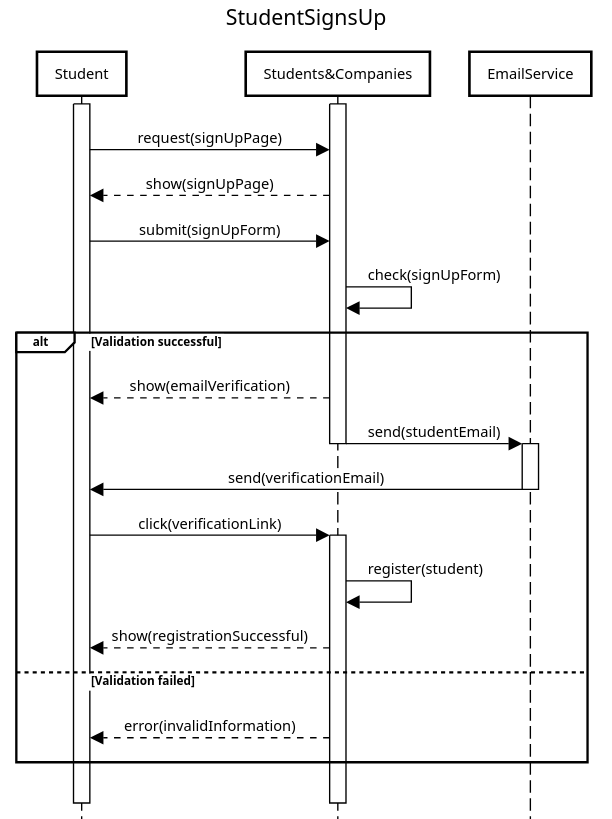
\includegraphics[width=0.75\textwidth]{../../assets/sequence-diagrams/use-cases/StudentSignsUp.png}
    }
\end{figure}

\item \subsubsection{CompanySignsUp}

\begin{figure}[H]
    \centering
    \fcolorbox{black}{white}{
        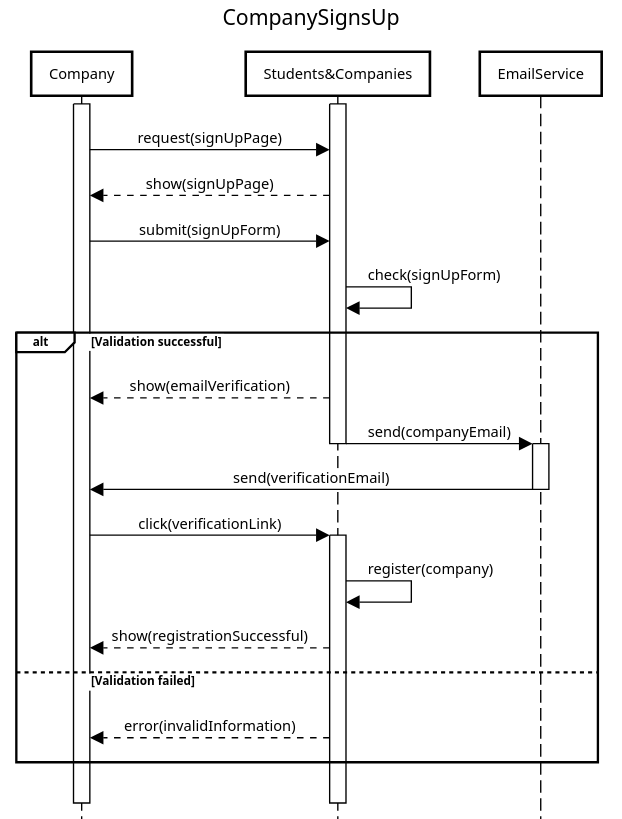
\includegraphics[width=0.75\textwidth]{../../assets/sequence-diagrams/use-cases/CompanySignsUp.png}
    }
\end{figure}

\item \subsubsection{UserLogsIn}

\begin{figure}[H]
    \centering
    \fcolorbox{black}{white}{
        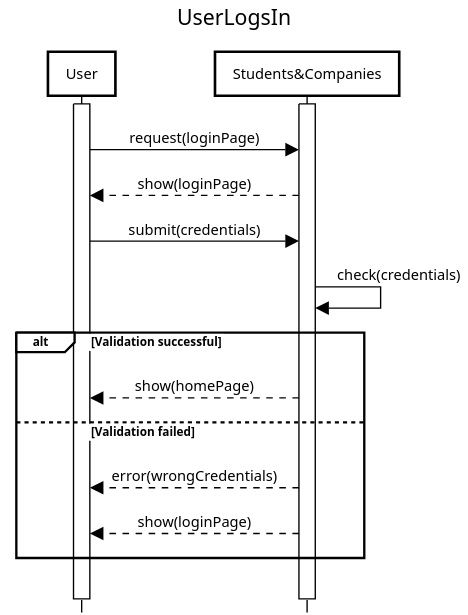
\includegraphics[width=0.5\textwidth]{../../assets/sequence-diagrams/use-cases/UserLogsIn.png}
    }
\end{figure}

\item \subsubsection{StudentUploadsCV}

\begin{figure}[H]
    \centering
    \fcolorbox{black}{white}{
        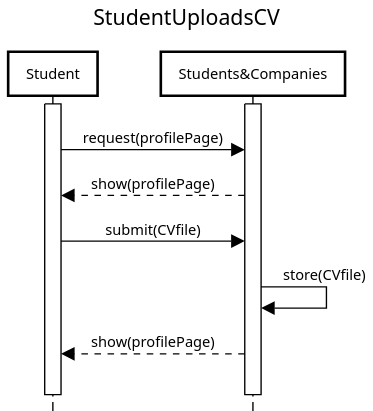
\includegraphics[width=0.5\textwidth]{../../assets/sequence-diagrams/use-cases/StudentUploadsCV.png}
    }
\end{figure}

\item \subsubsection{CompanyCreatesAdvertisement}

\begin{figure}[H]
    \centering
    \fcolorbox{black}{white}{
        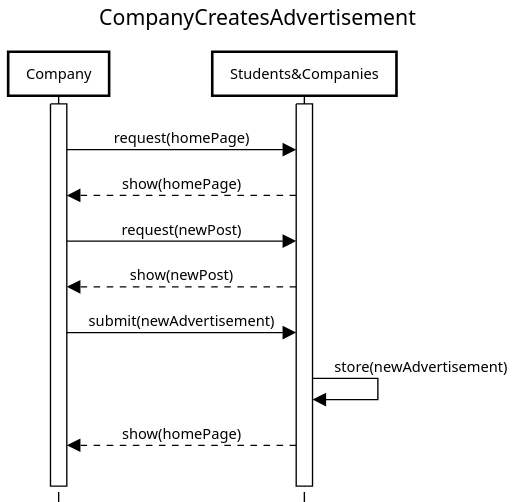
\includegraphics[width=0.5\textwidth]{../../assets/sequence-diagrams/use-cases/CompanyCreatesAdvertisement.png}
    }
\end{figure}

\item \subsubsection{StudentVisualizesAdvertisements}

\begin{figure}[H]
    \centering
    \fcolorbox{black}{white}{
        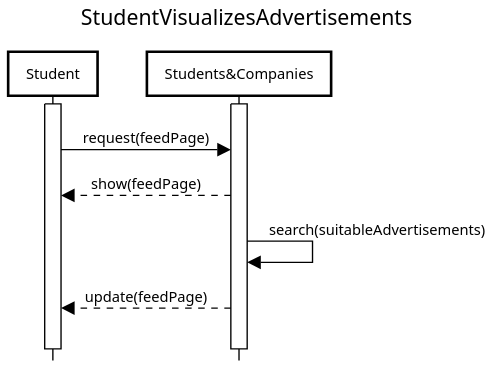
\includegraphics[width=0.5\textwidth]{../../assets/sequence-diagrams/use-cases/StudentVisualizesAdvertisements.png}
    }
\end{figure}

\item \subsubsection{CompanyVisualizesCandidates}

\begin{figure}[H]
    \centering
    \fcolorbox{black}{white}{
        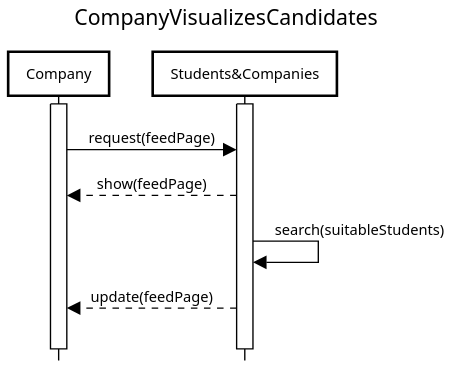
\includegraphics[width=0.5\textwidth]{../../assets/sequence-diagrams/use-cases/CompanyVisualizesCandidates.png}
    }
\end{figure}

\item \subsubsection{CompanyCreatesQuestionnaire}

\begin{figure}[H]
    \centering
    \fcolorbox{black}{white}{
        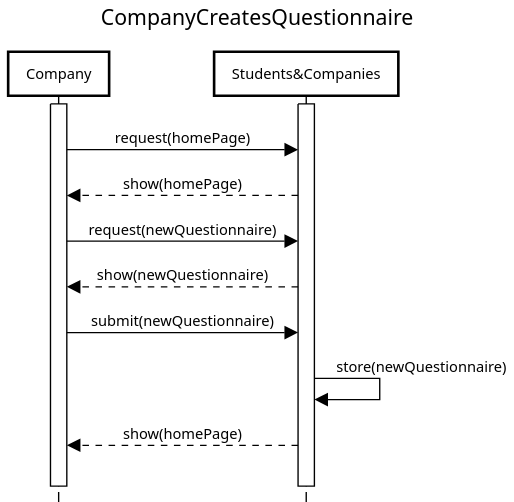
\includegraphics[width=0.5\textwidth]{../../assets/sequence-diagrams/use-cases/CompanyCreatesQuestionnaire.png}
    }
\end{figure}

\item \subsubsection{StudentFillsQuestionnaire}

\begin{figure}[H]
    \centering
    \fcolorbox{black}{white}{
        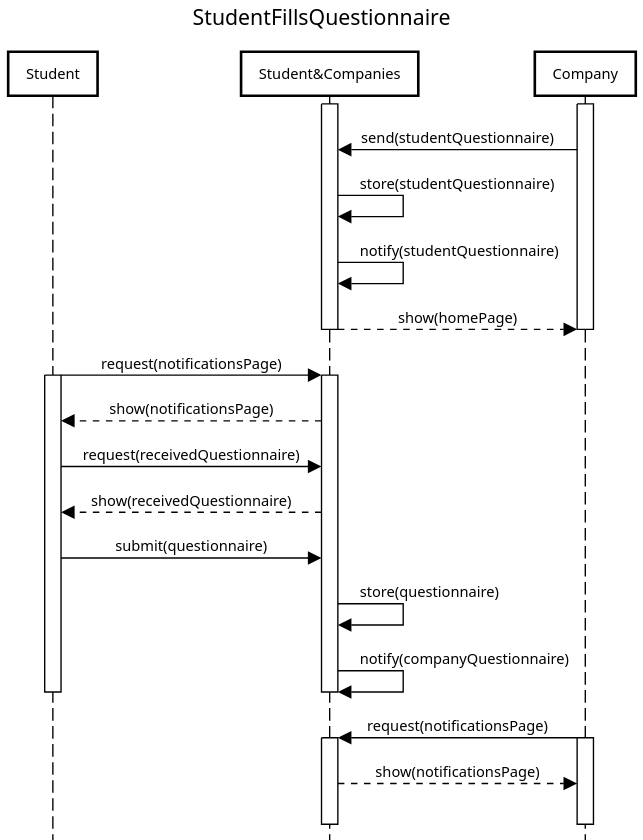
\includegraphics[width=0.75\textwidth]{../../assets/sequence-diagrams/use-cases/StudentFillsQuestionnaire.png}
    }
\end{figure}

\item \subsubsection{CompanyAcceptsStudentEnrollment}

\begin{figure}[H]
    \centering
    \fcolorbox{black}{white}{
        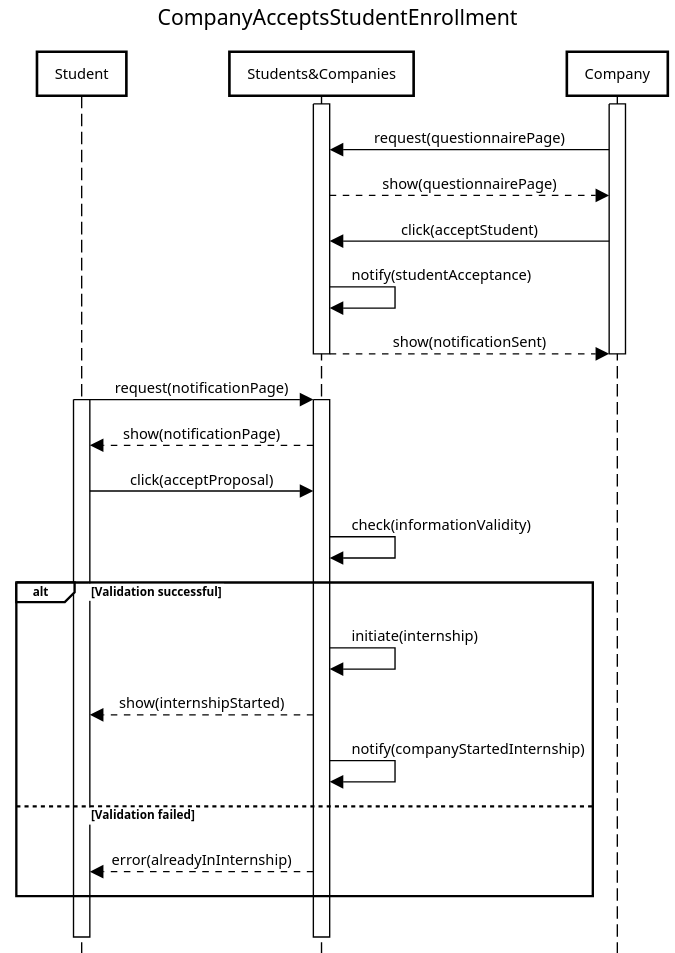
\includegraphics[width=0.75\textwidth]{../../assets/sequence-diagrams/use-cases/CompanyAcceptsStudentEnrollment.png}
    }
\end{figure}

\item \subsubsection{StudentVisualizesInternshipInformation}

\begin{figure}[H]
    \centering
    \fcolorbox{black}{white}{
        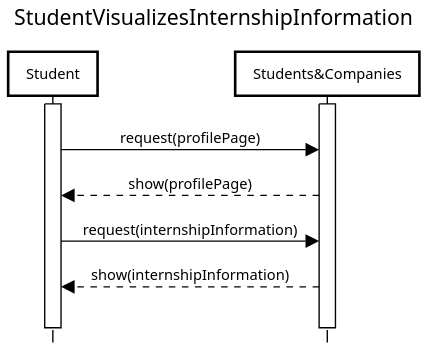
\includegraphics[width=0.5\textwidth]{../../assets/sequence-diagrams/use-cases/StudentVisualizesInternshipInformation.png}
    }
\end{figure}

\item \subsubsection{CompanyVisualizesInternshipsInformation}

\begin{figure}[H]
    \centering
    \fcolorbox{black}{white}{
        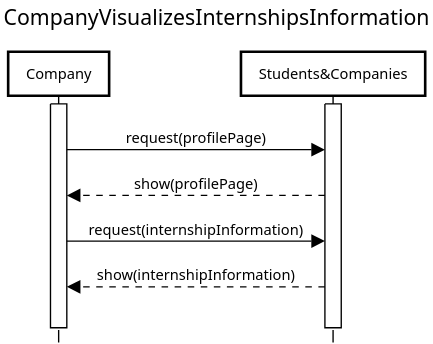
\includegraphics[width=0.5\textwidth]{../../assets/sequence-diagrams/use-cases/CompanyVisualizesInternshipsInformation.png}
    }
\end{figure}

\item \subsubsection{StudentSendsComplaint}

\begin{figure}[H]
    \centering
    \fcolorbox{black}{white}{
        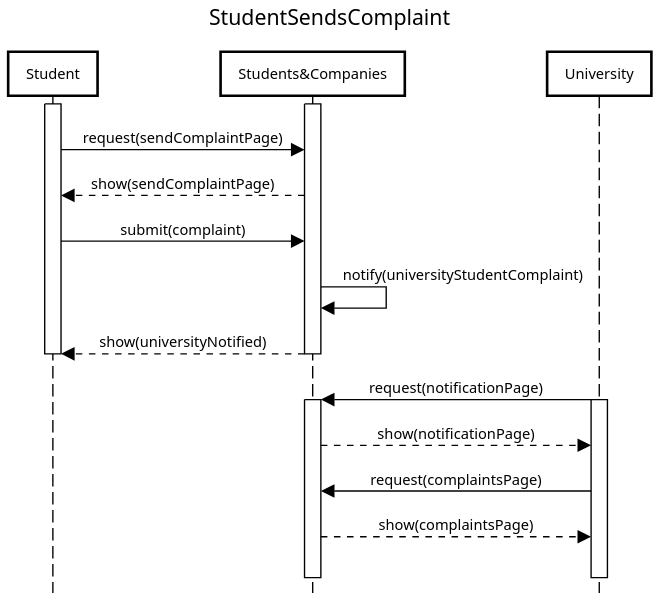
\includegraphics[width=0.75\textwidth]{../../assets/sequence-diagrams/use-cases/StudentSendsComplaint.png}
    }
\end{figure}

\item \subsubsection{CompanySendsComplaint}

\begin{figure}[H]
    \centering
    \fcolorbox{black}{white}{
        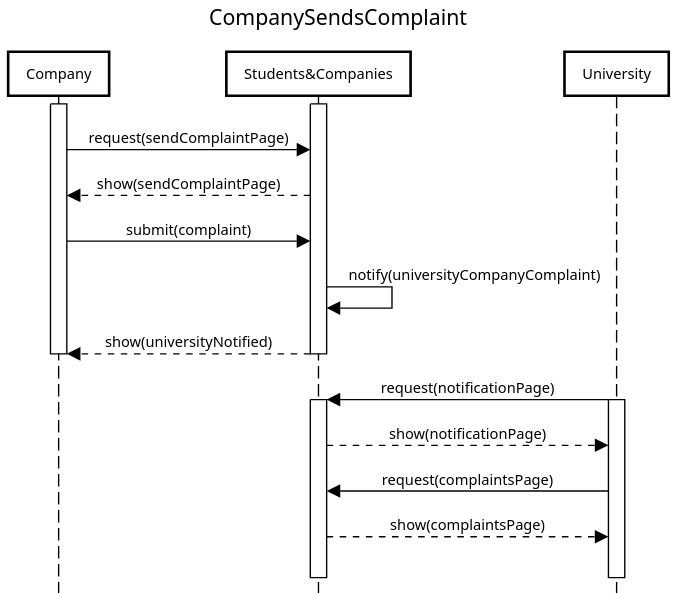
\includegraphics[width=0.75\textwidth]{../../assets/sequence-diagrams/use-cases/CompanySendsComplaint.png}
    }
\end{figure}

\item \subsubsection{UniversityVisualizesComplaints}

\begin{figure}[H]
    \centering
    \fcolorbox{black}{white}{
        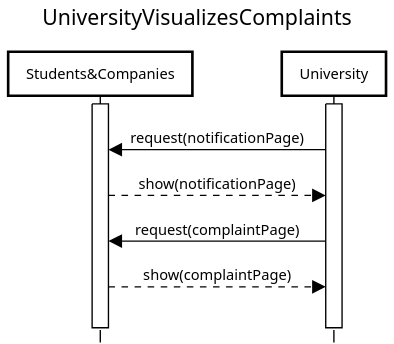
\includegraphics[width=0.5\textwidth]{../../assets/sequence-diagrams/use-cases/UniversityVisualizesComplaints.png}
    }
\end{figure}

\item \subsubsection{UniversityEndsInternship}

\begin{figure}[H]
    \centering
    \fcolorbox{black}{white}{
        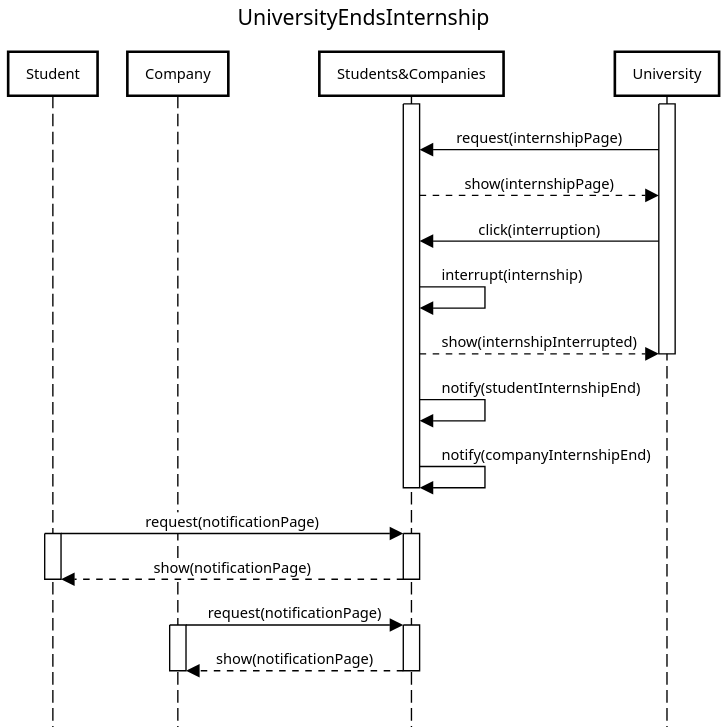
\includegraphics[width=0.75\textwidth]{../../assets/sequence-diagrams/use-cases/UniversityEndsInternship.png}
    }
\end{figure}

\item \subsubsection{InternshipExpires}

\begin{figure}[H]
    \centering
    \fcolorbox{black}{white}{
        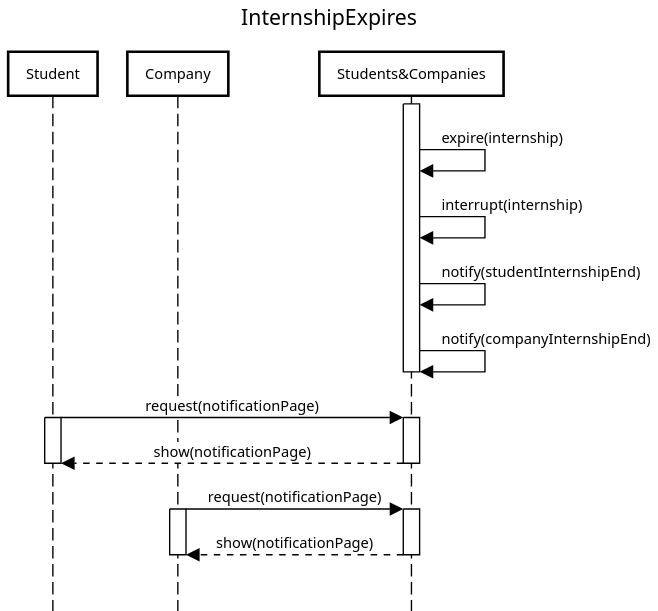
\includegraphics[width=0.75\textwidth]{../../assets/sequence-diagrams/use-cases/InternshipExpires.png}
    }
\end{figure}

\item \subsubsection{ParticipantFillsFeedbackForm}

\begin{figure}[H]
    \centering
    \fcolorbox{black}{white}{
        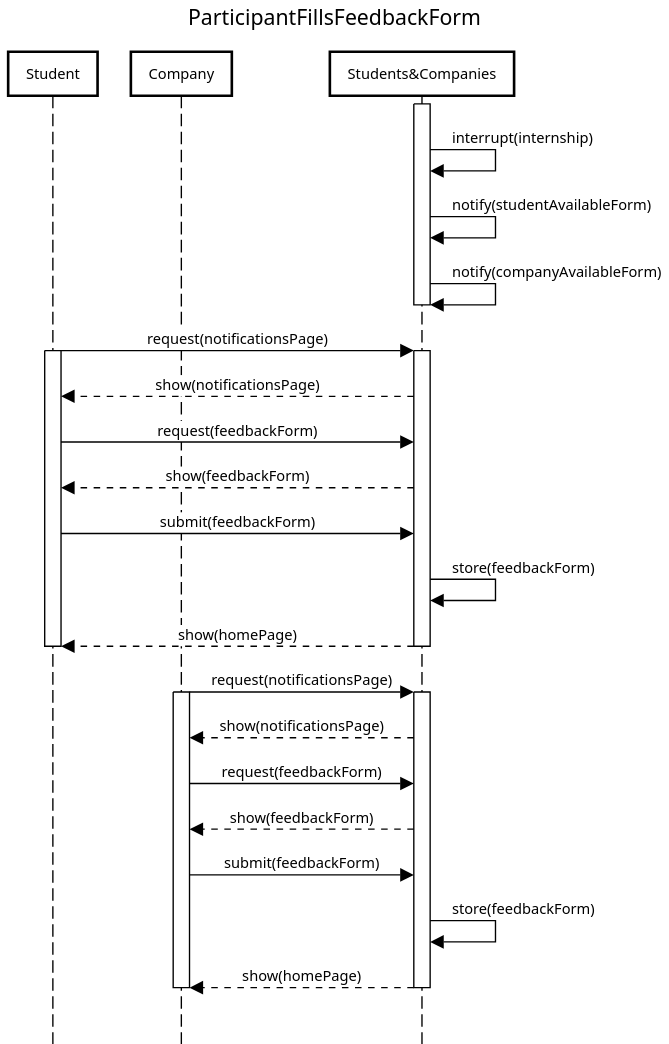
\includegraphics[width=0.75\textwidth]{../../assets/sequence-diagrams/use-cases/ParticipantFillsFeedbackForm.png}
    }
\end{figure}

\end{enumerate}

\subsection{Use cases mapping}

\begin{table}[H]
    \centering
    \begin{tabular}{|l|m{10cm}|}
        \hline \multicolumn{2}{|c|}{\textbf{Goal 1}} \\
        \hline \textbf{G1} & Allow registered students to search and enroll for internship opportunities. \\
        \hline \textbf{D1} & The user must have a working internet connection. \\
        \hline \textbf{D2} & The user must have provided valid personal information. \\
        %\hline \textbf{D3} & The student must be registered to a university. \\
        %\hline \textbf{D4} & The university must have provided an organization mail to the student. \\
        %\hline \textbf{R1} & The system must allow an unregistered student to sign up.\\
        %\hline \textbf{R2} & The system must allow an unregistered company to sign up. \\
        %\hline \textbf{R3} & The system must allow an unregistered university to sign up. \\
        \hline \textbf{R4} & The system must allow a registered user to log in. \\
        \hline \textbf{R5} & The system must allow a registered student to fill in and edit its personal information. \\
        \hline \textbf{R6} & The system must allow a registered student to upload its CV. \\
        \hline \textbf{R7} & The system must allow a registered company to post an internship project. \\
        \hline \textbf{R8} & The system must allow a registered student to visualize a list of open internship projects. \\
        %\hline \textbf{R9} & The system must allow a registered company to visualize a list of eligible students. \\
        \hline \textbf{R10} & The system must allow a registered student to make and enrollment request to an internship project. \\
        \hline \textbf{R11} & The system must allow a registered company to build custom made questionnaires. \\
        \hline \textbf{R12} & The system must allow a registered company to send questionnaires to students. \\
        \hline \textbf{R13} & The system must allow a registered student to fill in the questionnaire. \\
        \hline \textbf{R14} & The system must allow a registered company to accept students enrollment requests. \\
        %\hline \textbf{R15} & The system must allow a registered student to see their ongoing internship information. \\
        %\hline \textbf{R16} & The system must allow a registered company to see their ongoing internships information. \\
        %\hline \textbf{R17} & The system must allow a registered university to see their students' ongoing internship information. \\
        %\hline \textbf{R18} & The system must allow a registered student to send complaints to the university. \\
        %\hline \textbf{R19} & The system must allow a registered company to send complaints to the university. \\
        %\hline \textbf{R20} & The system must allow a registered university to visualize complaints it received. \\
        %\hline \textbf{R21} & The system must allow a registered university to end an ongoing internship of its student. \\
        \hline \textbf{R22} & The system must allow a registered student to fill in a feedback form when the internship ends. \\
        %\hline \textbf{R23} & The system must allow a registered company to fill in a feedback form when the internship ends. \\
        %\hline \textbf{R24} & The system must allow a registered student to visualize a list of suggested internships. \\
        %\hline \textbf{R25} & The system must allow a registered company to visualize a list of suggested students. \\
        \hline \textbf{R26} & The system must allow a registered student to be notified about recommended internship. \\
        %\hline \textbf{R27} & The system must allow a registered company to be notified about recommended students. \\
        \hline
    \end{tabular}
\end{table}

\begin{table}[H]
    \centering
    \begin{tabular}{|l|m{10cm}|}
        \hline \multicolumn{2}{|c|}{\textbf{Goal 2}} \\
        \hline \textbf{G2} & Allow registered companies to advertise internship project opportunities. \\
        \hline \textbf{D1} & The user must have a working internet connection. \\
        \hline \textbf{D2} & The user must have provided valid personal information. \\
        %\hline \textbf{D3} & The student must be registered to a university. \\
        %\hline \textbf{D4} & The university must have provided an organization mail to the student. \\
        %\hline \textbf{R1} & The system must allow an unregistered student to sign up.\\
        %\hline \textbf{R2} & The system must allow an unregistered company to sign up. \\
        %\hline \textbf{R3} & The system must allow an unregistered university to sign up. \\
        \hline \textbf{R4} & The system must allow a registered user to log in. \\
        %\hline \textbf{R5} & The system must allow a registered student to fill in and edit its personal information. \\
        %\hline \textbf{R6} & The system must allow a registered student to upload its CV. \\
        \hline \textbf{R7} & The system must allow a registered company to post an internship project. \\
        %\hline \textbf{R8} & The system must allow a registered student to visualize a list of open internship projects. \\
        \hline \textbf{R9} & The system must allow a registered company to visualize a list of eligible students. \\
        %\hline \textbf{R10} & The system must allow a registered student to make and enrollment request to an internship project. \\
        %\hline \textbf{R11} & The system must allow a registered company to build custom made questionnaires. \\
        %\hline \textbf{R12} & The system must allow a registered company to send questionnaires to students. \\
        %\hline \textbf{R13} & The system must allow a registered student to fill in the questionnaire. \\
        %\hline \textbf{R14} & The system must allow a registered company to accept students enrollment requests. \\
        %\hline \textbf{R15} & The system must allow a registered student to see their ongoing internship information. \\
        %\hline \textbf{R16} & The system must allow a registered company to see their ongoing internships information. \\
        %\hline \textbf{R17} & The system must allow a registered university to see their students' ongoing internship information. \\
        %\hline \textbf{R18} & The system must allow a registered student to send complaints to the university. \\
        %\hline \textbf{R19} & The system must allow a registered company to send complaints to the university. \\
        %\hline \textbf{R20} & The system must allow a registered university to visualize complaints it received. \\
        %\hline \textbf{R21} & The system must allow a registered university to end an ongoing internship of its student. \\
        %\hline \textbf{R22} & The system must allow a registered student to fill in a feedback form when the internship ends. \\
        %\hline \textbf{R23} & The system must allow a registered company to fill in a feedback form when the internship ends. \\
        \hline \textbf{R24} & The system must allow a registered student to visualize a list of suggested internships. \\
        \hline \textbf{R25} & The system must allow a registered company to visualize a list of suggested students. \\
        \hline \textbf{R26} & The system must allow a registered student to be notified about recommended internship. \\
        \hline \textbf{R27} & The system must allow a registered company to be notified about recommended students. \\
        \hline
    \end{tabular}
\end{table}

\begin{table}[H]
    \centering
    \begin{tabular}{|l|m{10cm}|}
        \hline \multicolumn{2}{|c|}{\textbf{Goal 3}} \\
        \hline \textbf{G3} & Allow registered universities to monitor their students ongoing internship and manage complaints. \\
        \hline \textbf{D1} & The user must have a working internet connection. \\
        \hline \textbf{D2} & The user must have provided valid personal information. \\
        \hline \textbf{D3} & The student must be registered to a university. \\
        \hline \textbf{D4} & The university must have provided an organization mail to the student. \\
        \hline \textbf{R1} & The system must allow an unregistered student to sign up.\\
        \hline \textbf{R2} & The system must allow an unregistered company to sign up. \\
        %\hline \textbf{R3} & The system must allow an unregistered university to sign up. \\
        \hline \textbf{R4} & The system must allow a registered user to log in. \\
        %\hline \textbf{R5} & The system must allow a registered student to fill in and edit its personal information. \\
        %\hline \textbf{R6} & The system must allow a registered student to upload its CV. \\
        %\hline \textbf{R7} & The system must allow a registered company to post an internship project. \\
        %\hline \textbf{R8} & The system must allow a registered student to visualize a list of open internship projects. \\
        %\hline \textbf{R9} & The system must allow a registered company to visualize a list of eligible students. \\
        %\hline \textbf{R10} & The system must allow a registered student to make and enrollment request to an internship project. \\
        %\hline \textbf{R11} & The system must allow a registered company to build custom made questionnaires. \\
        %\hline \textbf{R12} & The system must allow a registered company to send questionnaires to students. \\
        %\hline \textbf{R13} & The system must allow a registered student to fill in the questionnaire. \\
        %\hline \textbf{R14} & The system must allow a registered company to accept students enrollment requests. \\
        %\hline \textbf{R15} & The system must allow a registered student to see their ongoing internship information. \\
        %\hline \textbf{R16} & The system must allow a registered company to see their ongoing internships information. \\
        \hline \textbf{R17} & The system must allow a registered university to see their students' ongoing internship information. \\
        \hline \textbf{R18} & The system must allow a registered student to send complaints to the university. \\
        \hline \textbf{R19} & The system must allow a registered company to send complaints to the university. \\
        \hline \textbf{R20} & The system must allow a registered university to visualize complaints it received. \\
        \hline \textbf{R21} & The system must allow a registered university to end an ongoing internship of its student. \\
        \hline \textbf{R22} & The system must allow a registered student to fill in a feedback form when the internship ends. \\
        \hline \textbf{R23} & The system must allow a registered company to fill in a feedback form when the internship ends. \\
        %\hline \textbf{R24} & The system must allow a registered student to visualize a list of suggested internships. \\
        %\hline \textbf{R25} & The system must allow a registered company to visualize a list of suggested students. \\
        %\hline \textbf{R26} & The system must allow a registered student to be notified about recommended internship. \\
        %\hline \textbf{R27} & The system must allow a registered company to be notified about recommended students. \\
        \hline
    \end{tabular}
\end{table}

\begin{table}[H]
    \centering
    \begin{tabular}{|l|m{10cm}|}
        \hline \multicolumn{2}{|c|}{\textbf{Goal 4}} \\
        \hline \textbf{G4} & Support companies in the selection process by providing students with custom-made questionnaires. \\
        \hline \textbf{D1} & The user must have a working internet connection. \\
        \hline \textbf{D2} & The user must have provided valid personal information. \\
        %\hline \textbf{D3} & The student must be registered to a university. \\
        %\hline \textbf{D4} & The university must have provided an organization mail to the student. \\
        %\hline \textbf{R1} & The system must allow an unregistered student to sign up.\\
        %\hline \textbf{R2} & The system must allow an unregistered company to sign up. \\
        %\hline \textbf{R3} & The system must allow an unregistered university to sign up. \\
        \hline \textbf{R4} & The system must allow a registered user to log in. \\
        %\hline \textbf{R5} & The system must allow a registered student to fill in and edit its personal information. \\
        %\hline \textbf{R6} & The system must allow a registered student to upload its CV. \\
        %\hline \textbf{R7} & The system must allow a registered company to post an internship project. \\
        %\hline \textbf{R8} & The system must allow a registered student to visualize a list of open internship projects. \\
        \hline \textbf{R9} & The system must allow a registered company to visualize a list of eligible students. \\
        %\hline \textbf{R10} & The system must allow a registered student to make and enrollment request to an internship project. \\
        \hline \textbf{R11} & The system must allow a registered company to build custom made questionnaires. \\
        \hline \textbf{R12} & The system must allow a registered company to send questionnaires to students. \\
        %\hline \textbf{R13} & The system must allow a registered student to fill in the questionnaire. \\
        \hline \textbf{R14} & The system must allow a registered company to accept students enrollment requests. \\
        %\hline \textbf{R15} & The system must allow a registered student to see their ongoing internship information. \\
        %\hline \textbf{R16} & The system must allow a registered company to see their ongoing internships information. \\
        %\hline \textbf{R17} & The system must allow a registered university to see their students' ongoing internship information. \\
        %\hline \textbf{R18} & The system must allow a registered student to send complaints to the university. \\
        %\hline \textbf{R19} & The system must allow a registered company to send complaints to the university. \\
        %\hline \textbf{R20} & The system must allow a registered university to visualize complaints it received. \\
        %\hline \textbf{R21} & The system must allow a registered university to end an ongoing internship of its student. \\
        %\hline \textbf{R22} & The system must allow a registered student to fill in a feedback form when the internship ends. \\
        %\hline \textbf{R23} & The system must allow a registered company to fill in a feedback form when the internship ends. \\
        %\hline \textbf{R24} & The system must allow a registered student to visualize a list of suggested internships. \\
        %\hline \textbf{R25} &The system must allow a registered company to visualize a list of suggested students. \\
        %\hline \textbf{R26} & The system must allow a registered student to be notified about recommended internship. \\
        %\hline \textbf{R27} & The system must allow a registered company to be notified about recommended students. \\
        \hline
    \end{tabular}
\end{table}

\begin{table}[H]
    \centering
    \begin{tabular}{|l|m{10cm}|}
        \hline \multicolumn{2}{|c|}{\textbf{Goal 5}} \\
        \hline \textbf{G5} & Ease matching by notifying students of relevant internships and companies for suitable candidates. \\
        \hline \textbf{D1} & The user must have a working internet connection. \\
        \hline \textbf{D2} & The user must have provided valid personal information. \\
        \hline \textbf{D3} & The student must be registered to a university. \\
        \hline \textbf{D4} & The university must have provided an organization mail to the student. \\
        \hline \textbf{R1} & The system must allow an unregistered student to sign up.\\
        \hline \textbf{R2} & The system must allow an unregistered company to sign up. \\
        %\hline \textbf{R3} & The system must allow an unregistered university to sign up. \\
        \hline \textbf{R4} & The system must allow a registered user to log in. \\
        \hline \textbf{R5} & The system must allow a registered student to fill in and edit its personal information. \\
        \hline \textbf{R6} & The system must allow a registered student to upload its CV. \\
        \hline \textbf{R7} & The system must allow a registered company to post an internship project. \\
        \hline \textbf{R8} & The system must allow a registered student to visualize a list of open internship projects. \\
        \hline \textbf{R9} & The system must allow a registered company to visualize a list of eligible students. \\
        \hline \textbf{R10} & The system must allow a registered student to make and enrollment request to an internship project. \\
        \hline \textbf{R11} & The system must allow a registered company to build custom made questionnaires. \\
        \hline \textbf{R12} & The system must allow a registered company to send questionnaires to students. \\
        \hline \textbf{R13} & The system must allow a registered student to fill in the questionnaire. \\
        \hline \textbf{R14} & The system must allow a registered company to accept students enrollment requests. \\
        \hline \textbf{R15} & The system must allow a registered student to see their ongoing internship information. \\
        \hline \textbf{R16} & The system must allow a registered company to see their ongoing internships information. \\
        %\hline \textbf{R17} & The system must allow a registered university to see their students' ongoing internship information. \\
        %\hline \textbf{R18} & The system must allow a registered student to send complaints to the university. \\
        %\hline \textbf{R19} & The system must allow a registered company to send complaints to the university. \\
        %\hline \textbf{R20} & The system must allow a registered university to visualize complaints it received. \\
        %\hline \textbf{R21} & The system must allow a registered university to end an ongoing internship of its student. \\
        \hline \textbf{R22} & The system must allow a registered student to fill in a feedback form when the internship ends. \\
        \hline \textbf{R23} & The system must allow a registered company to fill in a feedback form when the internship ends. \\
        \hline \textbf{R24} & The system must allow a registered student to visualize a list of suggested internships. \\
        \hline \textbf{R25} & The system must allow a registered company to visualize a list of suggested students. \\
        \hline \textbf{R26} & The system must allow a registered student to be notified about recommended internship. \\
        \hline \textbf{R27} & The system must allow a registered company to be notified about recommended students. \\
        \hline
    \end{tabular}
\end{table}

\begin{table}[H]
    \centering
    \begin{tabular}{|l|m{10cm}|}
        \hline \multicolumn{2}{|c|}{\textbf{Goal 6}} \\
        \hline \textbf{G6} & Provide suggestions to both parties to refine their submissions. \\
        \hline \textbf{D1} & The user must have a working internet connection. \\
        \hline \textbf{D2} & The user must have provided valid personal information. \\
        %\hline \textbf{D3} & The student must be registered to a university. \\
        %\hline \textbf{D4} & The university must have provided an organization mail to the student. \\
        %\hline \textbf{R1} & The system must allow an unregistered student to sign up.\\
        %\hline \textbf{R2} & The system must allow an unregistered company to sign up. \\
        %\hline \textbf{R3} & The system must allow an unregistered university to sign up. \\
        \hline \textbf{R4} & The system must allow a registered user to log in. \\
        \hline \textbf{R5} & The system must allow a registered student to fill in and edit its personal information. \\
        \hline \textbf{R6} & The system must allow a registered student to upload its CV. \\
        \hline \textbf{R7} & The system must allow a registered company to post an internship project. \\
        \hline \textbf{R8} & The system must allow a registered student to visualize a list of open internship projects. \\
        \hline \textbf{R9} & The system must allow a registered company to visualize a list of eligible students. \\
        %\hline \textbf{R10} & The system must allow a registered student to make and enrollment request to an internship project. \\
        %\hline \textbf{R11} & The system must allow a registered company to build custom made questionnaires. \\
        %\hline \textbf{R12} & The system must allow a registered company to send questionnaires to students. \\
        %\hline \textbf{R13} & The system must allow a registered student to fill in the questionnaire. \\
        %\hline \textbf{R14} & The system must allow a registered company to accept students enrollment requests. \\
        %\hline \textbf{R15} & The system must allow a registered student to see their ongoing internship information. \\
        %\hline \textbf{R16} & The system must allow a registered company to see their ongoing internships information. \\
        %\hline \textbf{R17} & The system must allow a registered university to see their students' ongoing internship information. \\
        %\hline \textbf{R18} & The system must allow a registered student to send complaints to the university. \\
        %\hline \textbf{R19} & The system must allow a registered company to send complaints to the university. \\
        %\hline \textbf{R20} & The system must allow a registered university to visualize complaints it received. \\
        %\hline \textbf{R21} & The system must allow a registered university to end an ongoing internship of its student. \\
        %\hline \textbf{R22} & The system must allow a registered student to fill in a feedback form when the internship ends. \\
        %\hline \textbf{R23} & The system must allow a registered company to fill in a feedback form when the internship ends. \\
        \hline \textbf{R24} & The system must allow a registered student to visualize a list of suggested internships. \\
        \hline \textbf{R25} & The system must allow a registered company to visualize a list of suggested students. \\
        \hline \textbf{R26} & The system must allow a registered student to be notified about recommended internship. \\
        \hline \textbf{R27} & The system must allow a registered company to be notified about recommended students. \\
        \hline
    \end{tabular}
\end{table}

\section{Performance requirements}

Given the non-critical nature of the system, there are no overly stringent performance requirements.
However, the system strives to satisfy the following requirements in order to offer the best user experience.

\subsection{Specific requirements}

\begin{enumerate}[label=\textbf{SR\arabic* -}]
    \item The system should handle at least 1000 user requests per second.
    \item The system should respond to web page requests in under 2 seconds.
    \item The system should let users sign up within 5 seconds.
    \item The system should let users log in within 2 seconds.
    \item The system should let users access their profile information within 2 seconds.
    \item The system should let students upload their CV within 5 seconds.
    \item The system should let companies post advertisements within 2 seconds.
    \item The system should let students retrieve an advertisement project list within 2 seconds.
    \item The system should let companies retrieve a suitable student list within 2 seconds.
    \item The system should let students send an application request within 2 seconds.
    \item The system should let companies store a newly built custom questionnaire within 2 seconds.
    \item The system should let students submit a filled questionnaire within 2 seconds.
    \item The system should let companies accept a student enrollment within 2 seconds.
    \item The system should let students accept a company proposal within 2 seconds.
    \item The system should initiate an internship instance in under 5 seconds.
    \item The system should let users visualize ongoing internship information within 2 seconds.
    \item The system should let students and companies send complaints in under 2 seconds.
    \item The system should let universities visualize complaints within 2 seconds.
    \item The system should let universities end an internship within 2 seconds.
    \item The system should finish an internship instance in under 5 seconds.
    \item The system should let students and companies submit a filled feedback form within 2 seconds.
    \item The system should allow users to receive notifications in under 10 seconds.
    \item The system should find valid internship projects recommendations in under 5 seconds.
    \item The system should find valid suitable students in under 5 seconds.
    \item The system should find valid profile suggestions in under 5 seconds.
\end{enumerate}

\section{Design constraints}

This section outlines the constraints impacting design choices, including regulatory standards, technical limitations, and specific requirements.
These constraints guide compliance and design feasibility.

\subsection{Standards compliance}

Specications described in this document must be respected by the system.
The source code of the application must be commented and documented adequately.

Moreover, the system should respect the laws about privacy and data protection of the country in which it is used.

\subsection{Hardware limitations}

To access the system the user must have a device with a web browser and an internet connection.

%\subsection{Any other constraint}

\section{Software system attributes}

This section describes essential software attributes like performance, security, and maintainability, which define the quality and user experience of the system.

\subsection{Availability}

The system must operate continuously, ensuring 24/7 access with downtime below 1\%.
Any failure must be resolved within 1 hour to minimize service disruption.

\subsection{Reliability}

To maintain consistent performance, the system should be designed with high redundancy and fault tolerance, reducing the risk of critical failures.

\subsection{Security}

Data encryption is crucial to protect sensitive user information, including personal details and passwords.
All such data must be encrypted both in transit and at rest, ensuring it remains secure against unauthorized access.

Access control is enforced through a robust authentication and authorization mechanism that restricts data and functionality access according to user roles.
Passwords are securely hashed and stored, further safeguarding user credentials.

The system ensures responsible handling of personal data, requiring explicit user consent and implementing clear procedures for data protection.
Users have the right to access their data and request its deletion, promoting transparency and control over personal information.

To uphold high security standards, regular security audits and vulnerability assessments are scheduled.
These help identify and mitigate any emerging risks, continuously enhancing system security.

\subsection{Maintainability}

The system must be designed with maintainability in mind, ensuring that future updates, bug fixes, and feature enhancements can be implemented efficiently.

\subsection{Portability}

The system is designed to be platform-independent, accessible from any device with a web browser and an internet connection. The user interface is responsive and optimized for various screen sizes and resolutions.
